%% 
%% Copyright 2007, 2008, 2009 Elsevier Ltd
%% 
%% This file is part of the 'Elsarticle Bundle'.
%% ---------------------------------------------
%% 
%% It may be distributed under the conditions of the LaTeX Project Public
%% License, either version 1.2 of this license or (at your option) any
%% later version.  The latest version of this license is in
%%    http://www.latex-project.org/lppl.txt
%% and version 1.2 or later is part of all distributions of LaTeX
%% version 1999/12/01 or later.
%% 
%% The list of all files belonging to the 'Elsarticle Bundle' is
%% given in the file `manifest.txt'.
%% 

%% Template article for Elsevier's document class `elsarticle'
%% with numbered style bibliographic references
%% SP 2008/03/01

\documentclass[preprint,12pt,authoryear]{elsarticle}

%% Use the option review to obtain double line spacing
%% \documentclass[authoryear,preprint,review,12pt]{elsarticle}

%% Use the options 1p,twocolumn; 3p; 3p,twocolumn; 5p; or 5p,twocolumn
%% for a journal layout:
%% \documentclass[final,1p,times]{elsarticle}
%% \documentclass[final,1p,times,twocolumn]{elsarticle}
%% \documentclass[final,3p,times]{elsarticle}
%% \documentclass[final,3p,times,twocolumn]{elsarticle}
%% \documentclass[final,5p,times]{elsarticle}
%% \documentclass[final,5p,times,twocolumn]{elsarticle}

%% For including figures, graphicx.sty has been loaded in
%% elsarticle.cls. If you prefer to use the old commands
%% please give \usepackage{epsfig}

%% The amssymb package provides various useful mathematical symbols
\usepackage{amssymb}
\usepackage{amsmath}
\usepackage{url}
%% The amsthm package provides extended theorem environments
%% \usepackage{amsthm}

%% The lineno packages adds line numbers. Start line numbering with
%% \begin{linenumbers}, end it with \end{linenumbers}. Or switch it on
%% for the whole article with \linenumbers.
%%\usepackage{lineno}

%% Block of code for fixing corresponding author bug 
%% in elsarticle template... Don't really understand it
\makeatletter
\def\@author#1{\g@addto@macro\elsauthors{\normalsize%
    \def\baselinestretch{1}%
    \upshape\authorsep#1\unskip\textsuperscript{%
      \ifx\@fnmark\@empty\else\unskip\sep\@fnmark\let\sep=,\fi
      \ifx\@corref\@empty\else\unskip\sep\@corref\let\sep=,\fi
      }%
    \def\authorsep{\unskip,\space}%
    \global\let\@fnmark\@empty
    \global\let\@corref\@empty  %% Added
    \global\let\sep\@empty}%
    \@eadauthor={#1}
}
\makeatother
%% End block of weird code

%% Command for bold Greek symbols
\newcommand{\mitbf}[1]{\hbox{\mathversion{bold}$#1$}}

%in case I want to add detail to any derivation
\newif\ifdetail
\detailfalse
%\detailtrue

\journal{Physics of Earth and Planetary Interiors}

\begin{document}

\begin{frontmatter}

%% Title, authors and addresses

%% use the tnoteref command within \title for footnotes;
%% use the tnotetext command for theassociated footnote;
%% use the fnref command within \author or \address for footnotes;
%% use the fntext command for theassociated footnote;
%% use the corref command within \author for corresponding author footnotes;
%% use the cortext command for theassociated footnote;
%% use the ead command for the email address,
%% and the form \ead[url] for the home page:
%% \title{Title\tnoteref{label1}}
%% \tnotetext[label1]{}
%% \author{Name\corref{cor1}\fnref{label2}}
%% \ead{email address}
%% \ead[url]{home page}
%% \fntext[label2]{}
%% \cortext[cor1]{}
%% \address{Address\fnref{label3}}
%% \fntext[label3]{}

\title{Scaling rates of true polar wander in convecting planets and moons}

%% use optional labels to link authors explicitly to addresses:
%% \author[label1,label2]{}
%% \address[label1]{}
%% \address[label2]{}

\author{Ian Rose\corref{cor1}\fnref{ref1}}
\author{Bruce Buffett\fnref{ref1}}

\fntext[ref1]{University of California, Berkeley}
\cortext[cor1]{Corresponding author, \url{ian.rose@berkeley.edu}}

\address{}

\begin{abstract}
Mass redistribution in the convecting mantle of a planet can cause perturbations in its moment of inertia tensor. 
Conservation of angular momentum dictates that these perturbations can change the direction of the rotation vector of the planet, a process known as true polar wander (TPW). 
Although the existence of TPW on Earth is well-verified, its rate and magnitude over geologic time scales remain controversial. 
Here we present scaling analyses and numerical simulations of TPW due to mantle convection over a range of parameter space relevant to planetary interiors. 
For simple rotating convection, the most important parameters are the Rayleigh number, the rotation rate, and the size of relative density fluctuations (i.e. thermal expansivity times the temperature variations). 
We identify timescales for the growth of moment of inertia perturbations due to convection and for their relaxation due to true polar wander. 
These timescales, as well as the relative sizes of convective anomalies, control the rate and magnitude of TPW.
This analysis also clarifies the nature of so called ``inertial interchange'' TPW events, and when they are likely to occur.
Finally, we discuss implications for large-scale TPW in Earth's past, which has been suggested to be important for life and climate history.
\end{abstract}

\begin{keyword}
Rotational variations; polar wobble \sep
Paleomagnetism \sep
Models of interior structure \sep
Planetary interiors \sep
Convection currents and mantle plumes \sep
\PACS 91.10.Nj \sep 91.25.Ng \sep 91.35.Cb \sep 91.45.Bg \sep 91.45.Fj
%% keywords here, in the form: keyword \sep keyword

%% PACS codes here, in the form: \PACS code \sep code

%% MSC codes here, in the form: \MSC code \sep code
%% or \MSC[2008] code \sep code (2000 is the default)

\end{keyword}

\end{frontmatter}

%%\linenumbers

%%BEGINCLIP

\section{Introduction}
\label{sec:intro}

A rotating, quasistatic body like a planetary mantle will tend to spin about the axis of its maximum moment of inertia.
Convection in a planetary mantle continuously redistributes mass, which can change the moment of inertia tensor, necessitating a change in the spin axis of the planet to conserve angular momentum, a process known as true polar wander (TPW).

TPW was first considered in detail by \citet{darwin1887influence}, and the theory has been subsequently developed by many \citep[e.g.][]{munk1960rotation, goldreich1969some, ricard1993polar}. 
Despite this, the ability of internal mass anomalies to drive large-scale TPW remains controversial. 
Paleomagnetic data have been interpreted to require up to $3^\circ-12^\circ$/Myr rates of TPW \citep{mitchell2011sutton}, but the ability of the mantle to respond at such rates has been questioned \citep{tsai2007theoretical}.

The primary uncertainties in assigning a maximum TPW rate to a convecting planet are the size of convective anomalies, which drive the rotational adjustment, and the viscosity structure of the mantle, which retards it. 
These two uncertainties are not unrelated: they are both expected to be functions of the geometric and material properties of the mantle.
As such, they do not vary independently, and first-order questions about the propensity for planets to experience TPW remain: how are rates of TPW expected to vary with the vigor of convection? 
Are other planetary bodies more or less likely than Earth to experience TPW?  And are these rates expected to vary through Earth history?

These questions suggest that an approach rooted in dimensional analysis and fluid dynamics can clarify the rates and magnitudes of TPW.
Most previous studies coupling mantle convection models to polar wander calculations have done so with prescribed density perturbations \citep[e.g.][]{greff2004upwelling}, or prescribed moment of inertia variations \citep[e.g.][]{tsai2007theoretical, creveling2012mechanisms}. 
\citet{richards1999polar} coupled thermal convection models to a polar wander model, but did not address in detail the scaling relationships between the two.

Herein we perform a scaling analysis of rates of TPW for a minimal system of a rotating, convecting mantle,  which we support with numerical simulations.

\section{Rotational dynamics}
\label{sec:rotational_dynamics}

\subsection{The Liouville equation}
\label{sec:liouville}
Conservation of angular momentum for a torque-free system in a rotating reference frame requires

\begin{equation}
\frac{d \mathbf{H}}{dt} + \mitbf{\Omega} \times \mathbf{H} = 0
\label{eq:euler}
\end{equation}
where $\mathbf{H} = \mathbf{I} \cdot \mitbf{\Omega}$ is the angular momentum vector, $\mathbf{I}$ is the moment of inertia tensor, and $\mitbf{\Omega}$ is the angular velocity vector.
On a dynamic planet $\mathbf{I}$ may be a function of time, so to conserve angular momentum $\mitbf{\Omega}$ must be also vary with time.
In this case, Equation~\eqref{eq:euler} is often called the Liouville equation \citep[e.g.][]{munk1960rotation}.
For a slowly convecting fluid, such as a planetary mantle, the inertial term $\partial \mathbf{H} / \partial t$ is negligible, so we may solve the simplified quasistatic equations
\begin{equation}
\mitbf{\Omega } (t)\times ( \mathbf{I}(t) \cdot \mitbf{\Omega }(t) ) = 0.
\label{eq:quasistatic_liouville}
\end{equation}
Equation~\eqref{eq:quasistatic_liouville} indicates that $\mitbf{\Omega}$ and $\mathbf{H}$ are parallel, so a solution for $\mitbf{\Omega}(t)$ is equivalent to solving an eigenvalue problem for $\mathbf{I}(t)$, where the eigenvectors correspond to the principal axes and the eigenvalues correspond to the principal moments (where the most stable orientation of the planet corresponds to rotating about the largest principal axis).
In practice, this eigenvalue approach has been often used in previous studies for computing the spin axis of a planet \citep[e.g.][]{steinberger1997changes, roberts2007cause}.
The moment of inertia tensor in Equation~\eqref{eq:quasistatic_liouville} includes all contributions to the mass structure
of the planet, including the spherically symmetric mass distribution, rotational deformation, deformation due to self gravity, internal and surface density anomalies, and surface deflections due to density anomalies.
Here we are interested in contributions from mantle convection, so we restrict our attention to these processes.

For mantle convection problems the moment of inertia tensor is commonly separated into three parts \citep{sabadini1981pleistocene, spada1992excitation}:
\begin{equation}
I_{ij}(t) = I_0 \delta_{ij} + J_{ij}(t) + E_{ij}(t)
\label{eq:separation}
\end{equation}
where $I_0$ is the spherically symmetric reference moment, $J_{ij}$ is the contribution due to rotational deformation, and $E_{ij}$ is the contribution due to internal density anomalies, as well as the surface deflections caused by them.
If we plug this decomposition into Equation~\eqref{eq:quasistatic_liouville} the spherically symmetric part $I_0 \delta_{ij}$ drops out, and we are left with
\begin{equation}
\mathbf{\Omega} \times (\mathbf{J} \cdot \mitbf{\Omega}) = -\mitbf{\Omega} \times ( \mathbf{E} \cdot \mitbf{\Omega} ).
\label{eq:disequilibrium}
\end{equation}
This form of the quasistatic Liouville equation makes clear that the polar wander problem represents a balance between the mismatches
of the convective part of the moment of inertia ($\mathbf{E}$) and the rotational deformation part of the moment of inertia ($\mathbf{J}$).
Our goal is to characterize this balance from a perspective of scaling and fluid dynamics.

\subsection{A note on reference frames}
\label{sec:reference_frames}
True polar wander can be described in different reference frames, and this choice is fundamentally an arbitrary one.
However, certain aspects of the physics can be made much simpler by an appropriate choice of the reference frame.
In our treatment of TPW, we will refer to three different reference frames:
\begin{itemize}
\item First, there is the inertial, non-rotating frame corresponding to spatial coordinates that are fixed in time.
\item Second, there is the body-fixed (or geographic) frame.
By definition, the rotation of the body-fixed frame relative to the inertial frame is specified by $\mitbf{\Omega}$.
A terrestrial no-net-rotation or hotspot reference frame are common choices for the body-fixed frame.
Treatments of gravitational or rotational deformation of a planet are most naturally expressed in the body-fixed frame,
as described in Section~\ref{sec:rotational_deformation}.
\item Finally, there is the frame described by the principal axes of convective part of the moment of inertia $\mathbf{E}$,
which we will refer to as the ``$\mathbf{E}$-frame.'' 
Redistribution of mantle mass anomalies due to convection changes the principal axes of $\mathbf{E}$, 
causing the $\mathbf{E}$-frame to slowly rotate with respect to the geographic frame. We denote this drift 
by a rotation vector $\mitbf{\Psi}$ (see Section~\ref{sec:theta}).
\end{itemize}

These reference frames and vectors are illustrated in Figure~\ref{fig:reference_frames}.


\subsection{Rotational deformation}
\label{sec:rotational_deformation}

The part of the moment of inertia due to the elastic rotational deformation in the body-fixed frame 
is traditionally related to the degree-two part of the gravity field via MacCullagh's formula \citep{munk1960rotation}:
\begin{equation}
J_{ij} = \frac{k a^5}{3 G} \left( \Omega_i \Omega_j - \frac{1}{3} \Omega_q \Omega_q \delta_{ij} \right)
\label{eq:elastic_deformation}
\end{equation}
where $k$ is an elastic Love number, $a$ is the semimajor axis of the planet, and $G$ is the gravitational constant.
This result may be extended to a viscoelastic rheology via the viscoelastic correspondence principle \citep[e.g.][]{peltier1974impulse}:
\begin{equation}
J_{ij} = \frac{k(t) a^5}{3 G} * \left( \Omega_i \Omega_j - \frac{1}{3} \Omega_q \Omega_q \delta_{ij} \right)
\label{eq:viscoelastic_deformation}
\end{equation}
where $k$ is now a time-dependent viscoelastic Love number which is convolved with the time-dependent rotation vector.

The infinite-time limit of Equation~\eqref{eq:viscoelastic_deformation} for a 
constant rotation vector around the $z$-axis implies
\begin{equation}
\begin{aligned}
J_{zz} = C = &\frac{2}{3} \frac{k_f a^5 \Omega^2}{3 G} \\
J_{xx} = J_{yy} = A = -&\frac{1}{3} \frac{k_f a^5 \Omega^2}{3 G} \\
\end{aligned}
\end{equation}
where $C$ and $A$ are the polar and equatorial moments of inertia, respectively, 
and $k_f$ is the fluid limit of $k$. 
We can solve for $k_f$ in terms of $C-A$:
\begin{equation}
k_f = \frac{3 G (C-A)}{\Omega^2 a^5}.
\label{eq:fluid_love}
\end{equation}
This fluid-limit representation of the deformation does not allow for any disequilibrium between $J_{ij}$ and $E_{ij}$,
so it does not permit TPW.

\citet{ricard1993polar} obtain an approximation to Equation~\eqref{eq:viscoelastic_deformation} which retains its long-time behavior by entering the Laplace domain and truncating a Taylor series for $k(s)$ to first order.  
This introduces a new parameter, termed $T_1$, which can be seen as a weighted relaxation time for the system.  
This simple approximation in the Laplace domain allows for an analytical transformation back into the time domain, and neglecting second order terms in $\dot{\Omega}$ we find:
\begin{equation}
J_{ij} = \frac{k_f a^5}{3 G} \left( \Omega_i \Omega_j - \frac{1}{3} \Omega_q \Omega_q \delta_{ij} \right) -
 \frac{k_f a^5 T_1}{3G} \left(\dot{\Omega}_i \Omega_j + \Omega_i \dot{\Omega}_j - \frac{2}{3} \Omega_q \dot{\Omega}_q \delta_{ij} \right).
\label{eq:rotational_deformation}
\end{equation}
The two terms of this equation have simple interpretations.  
The first term corresponds to the fluid limit of rotational deformation (in the absence of any long-term elastic strength).  
The second term represents the lag in the moment of inertia due to the viscous adjustment of the rotational bulge, where $T_1$ is the characteristic time constant for this adjustment.
Since the first term represents the fluid limit of rotational deformation, it automatically satisfies Equation~\eqref{eq:quasistatic_liouville}, and hence does not contribute to the polar wander problem.

\subsection{The convective moment of inertia}
\label{sec:convective_moment}

The term on the right-hand side of Equation~\eqref{eq:disequilibrium} represents the moment of inertia due to internal density anomalies as well as the surface deflections due to them.
This part of the moment of inertia may also be parameterized using a viscoelastic Love number approach:
\begin{equation} 
\mathbf{E} = \left[ \delta(t) + k^L(t) \right] * \mathbf{C}
\end{equation}
where $k^L$ is an internal loading Love number representing the surface deflection due to density anomalies, 
and $C_{ij}$ is the moment of inertia due solely to the internal load.
Frequently the simplification is made that the timescale of the surface response is quick compared to the true polar wander timescale, and we may use the fluid limit geoid kernels \citep[e.g.][]{richards1984geoid}:  
\begin{equation}
E_{ij} = (1+k^L_f) C_{ij}.
\end{equation}
An alternative to the Love number formalism is to calculate to surface deflections directly using mantle convection simulations with a true free surface boundary condition.
A recent implementation of a free surface boundary condition in the CIG-sponsored mantle convection software \texttt{ASPECT} \citep{rose2016free}
permits more general treatments of mantle rheology.

\subsection{Rate of true polar wander}
\label{sec:tpw_rate}

We are in a position to address the rates of true polar wander for a given convective moment $\mathbf{E}$.
A considerable simplification occurs if we neglect secular changes in the rotation rate, and just consider changes in direction of the pole ($d \Omega^2 / dt = 2 {\Omega_i} \dot{ \Omega}_i = 0$)
Substituting Equation~\eqref{eq:rotational_deformation} into Equation~\eqref{eq:disequilibrium} we find
\begin{equation}
\frac{k_f a^5 T_1 \Omega^2}{3G}\mitbf{\Omega} \times \dot{\mitbf{\Omega} } = \mitbf{\Omega} \times \left( \mathbf{E} \cdot \mitbf{\Omega} \right).
\label{eq:liouville}
\end{equation}
Introducing a unit vector $\mitbf{\omega} = \mitbf{\Omega}/\|\mitbf{\Omega} \|$ and using Equation~\eqref{eq:fluid_love} for $k_f$,  we may solve this equation for $\dot{\mitbf{\omega}}$:
\begin{equation}
 \dot{\mitbf{\omega}}  = \frac{1}{(C-A)T_1} \left[ \mathbf{E} \cdot \mitbf{\omega} - \left( \mitbf{\omega} \cdot \mathbf{E} \cdot \mitbf{\omega}  \right) \mitbf{\omega} \right].
\label{eq:liouville_ode}
\end{equation}
Note that the quantity in brackets is similar in form to the shear stress on a plane in classical elastostatics.
This correspondence permits useful insights (see below).
Let $\dot{\Theta} = \vert \dot{\mitbf{\omega}} \vert$ denote the rate of polar wander.
Evaluating the scalar product $\dot{\Theta}^2 = \dot{\mitbf{\omega}} \cdot \dot{\mitbf{\omega}}$ gives
\begin{equation}
\dot{\Theta}^2 = \dot{\mitbf{\omega}}^2 = \frac{1}{(C-A)^2 T_1^2} \left[ (\mathbf{E}\cdot\mitbf{\omega})^2 - (\mitbf{\omega}\cdot\mathbf{E}\cdot\mitbf{\omega})^2 \right].
\label{eq:polar_wander_rate_tensor}
\end{equation}

\begin{figure*}
\centering
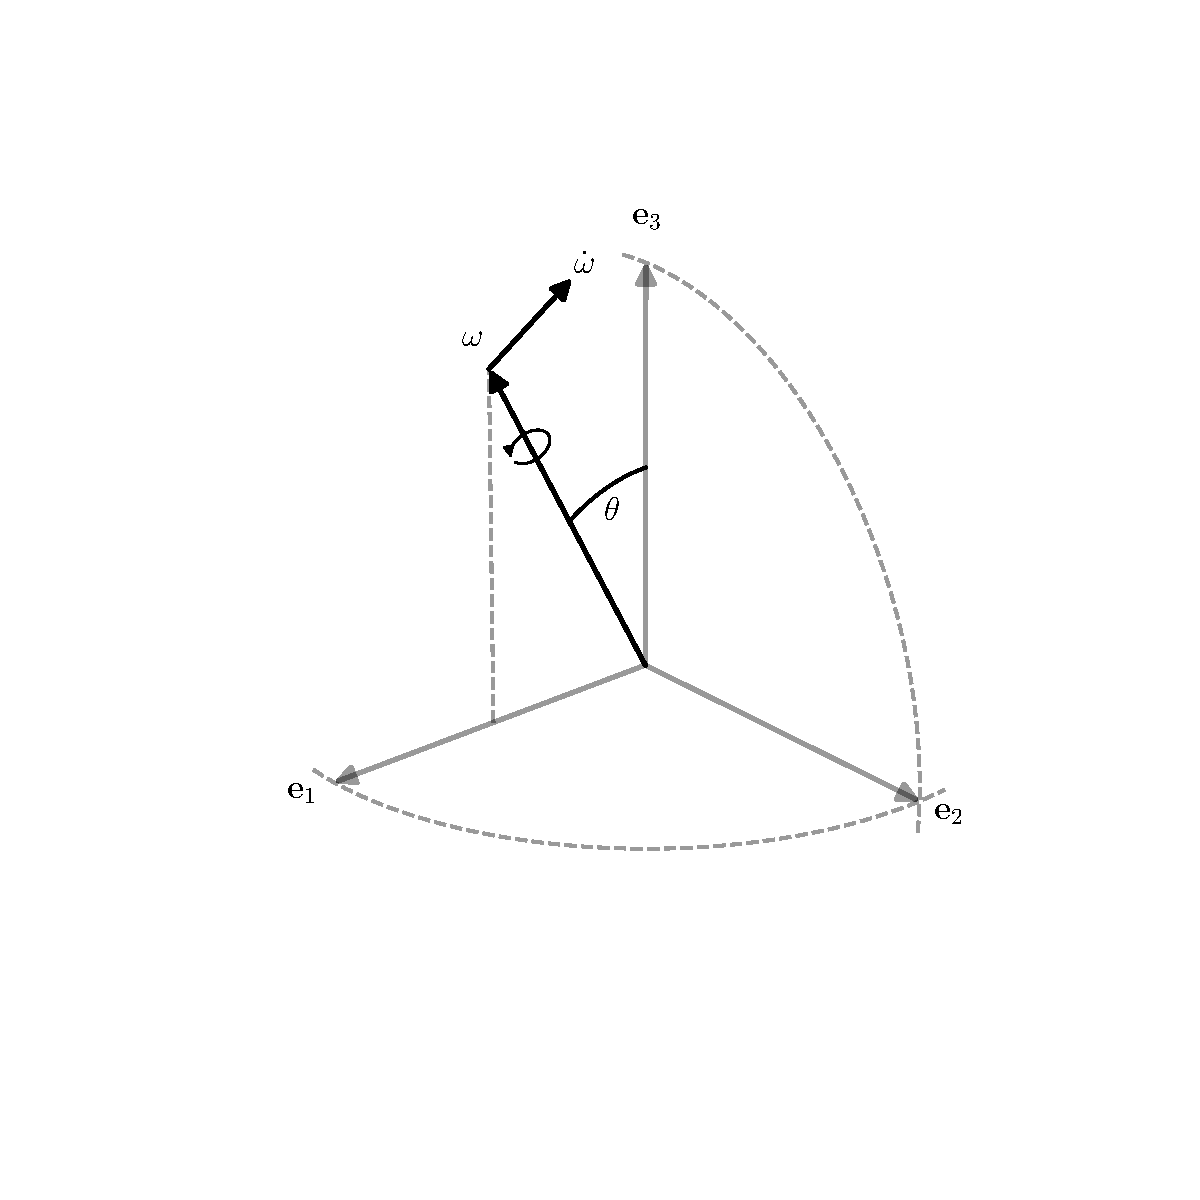
\includegraphics[width=0.9\textwidth]{figures/reference_frames.pdf}
\caption[Relevant vectors and angles for the TPW analysis.]{Relevant vectors and angles for the TPW analysis. The axes $\mathbf{e}_1$, $\mathbf{e}_2$, and $\mathbf{e}_3$ represent the principal axes of the convective moment of inertia $\mathbf{E}$, with associated eigenvalues $\lambda_1$, $\lambda_2$, and $\lambda_3$, respectively. Since the choice of geographic axes is arbitrary, we assume that at this instant the $\mathbf{E}$-frame and the geographic frames are colocated (though at future times they will not be). The angle $\theta$ represents the mismatch between the rotation axis $\mitbf{\omega}$ and the $\mathbf{e}_3$-axis. For illustration, we assume the longitude $\phi$ of the rotation axis is zero so $\mitbf{\omega}$ lies in the $\mathbf{e_1}$-$\mathbf{e_3}$ plane. True polar wander moves the rotation axis towards the $\mathbf{e}_3$-axis. We denote this motion by $\dot{\mitbf{\omega}}$ in the geographic frame. However, time-dependent convection in the mantle may cause a relative rotation between the geographic frame and the $\mathbf{E}$-frame. This relative rotation can be represented as a rotation around the axis $\mitbf{\Psi}$, which is defined by colatitude $\beta$ and longitude $\gamma$. The rotation around the $\mitbf{\Psi}$ axis contributes to the motion of $\mitbf{\omega}$ as seen in the $\mathbf{E}$-frame.  Further discussion of the reference frames and the relative rotation vector $\mitbf{\Psi}$ can be found in Sections~\ref{sec:reference_frames} and \ref{sec:theta}}
\label{fig:reference_frames}
\end{figure*}

Our goal is to quantify the polar wander rate $\dot{\Theta}$ due to a convective perturbation $\mathbf{E}$ in the moment of inertia. 
The rate defined by Equation~\eqref{eq:polar_wander_rate_tensor} is expressed in the body-fixed geographic frame, 
which is also the reference frame used to measure TPW. 
However, the physics of the right-hand-side of Equation~\eqref{eq:polar_wander_rate_tensor} 
is more naturally expressed in the reference frame of the principal axes of $\mathbf{E}$. 
In general the $\mathbf{E}$-frame rotates slowly with respect to the geographic frame, so the time derivative of $\omega$ is different in these two frames.
However, Equation~\eqref{eq:polar_wander_rate_tensor} is a scalar equation, which means it is invariant to rotations.
Therefore we can enter the coordinate system of the convective moment of inertia $\mathbf{E}$ 
with principal moments $\lambda_1 \le \lambda_2 \le \lambda_3$ and define the orientation of 
$\mitbf{\omega}$ in the $\mathbf{E}$-frame with colatitude $\theta$ and longitude $\phi$ (see Figure~\ref{fig:reference_frames}).
Plugging this description of $\mitbf{\omega}$ into Equation~\eqref{eq:polar_wander_rate_tensor},
and after some tedious algebra, we find
\ifdetail

And here is the tedious algebra.  Let the prefactors $\frac{1}{(C-A)T_1}$ be denoted by $A$.
We are interested in the rate of true polar wander, which is the angular change of the pole
per unit time. We can transform Equation~\eqref{eq:liouville_ode} into a scalar equation by dotting it
with $\dot{\mitbf{\omega}}$, since we are interested in the magnitude of the rate, rather than
the direction at the moment.

\begin{equation}
\begin{aligned}
\dot{\mitbf{\omega}} \cdot \dot{\mitbf{\omega}} &= 
A^2 \left[ \mathbf{E}\cdot \mitbf{\omega} - \left(\mitbf{\omega} \cdot \mathbf{E} \cdot \mitbf{\omega} \right)\mitbf{\omega}\right]
\cdot \left[ \mathbf{E}\cdot \mitbf{\omega} - \left(\mitbf{\omega} \cdot \mathbf{E} \cdot \mitbf{\omega} \right)\mitbf{\omega}\right] \\
\dot{\mitbf{\omega}}^2  &= 
A^2 \left[ \left(\mathbf{E}\cdot \mitbf{\omega}\right)\cdot \left(\mathbf{E}\cdot \mitbf{\omega}\right)
 - \left(\mitbf{\omega} \cdot \mathbf{E} \cdot \mitbf{\omega} \right) \left( \mitbf{\omega}\cdot \mathbf{E} \cdot \mitbf{\omega} \right) 
 - \left(\mitbf{\omega} \cdot \mathbf{E} \cdot \mitbf{\omega} \right) \left( \mitbf{\omega}\cdot \mathbf{E} \cdot \mitbf{\omega} \right) 
 + \left(\mitbf{\omega} \cdot \mathbf{E} \cdot \mitbf{\omega} \right)^2 \mitbf{\omega}\cdot \mitbf{\omega} 
\right]\\
\dot{\mitbf{\omega}}^2  &= 
A^2 \left[ \left(\mathbf{E}\cdot \mitbf{\omega}\right)^2
 - \left(\mitbf{\omega} \cdot \mathbf{E} \cdot \mitbf{\omega} \right)^2.
\right]\\
\end{aligned}
\end{equation}
Since this is a scalar equation, we can arbitrarily choose a coordinate system in which to evaluate it.
It is most convenient to choose the principal axes of $\mathbf{E}$, where
\begin{equation}
\mathbf{E} = 
\begin{bmatrix}
\lambda_1 & 0 & 0 \\
0 & \lambda_2 & 0 \\
0 & 0 & \lambda_3 \\
\end{bmatrix}
\end{equation}
\begin{equation}
\mitbf{\omega} = 
\begin{bmatrix}
\sin{\theta} \cos{\phi} \\
\sin{\theta} \sin{\phi} \\
\cos{\theta} \\
\end{bmatrix}.
\end{equation}

As a warm-up, consider the case where $\phi = 0$, then  
\begin{equation}
\mitbf{\omega} = 
\begin{bmatrix}
\sin{\theta}  \\
0 \\
\cos{\theta} \\
\end{bmatrix}
\end{equation}
We can evaluate some of the terms of the scalar equation for $\dot{\mitbf{\omega}}^2$:
\begin{equation}
\mathbf{E}\cdot \mitbf{\omega} = 
\begin{bmatrix}
\lambda_1 \sin{\theta} \\
0 \\
\lambda_3 \cos{\theta}
\end{bmatrix}
\end{equation}

\begin{equation}
\left(\mathbf{E}\cdot \mitbf{\omega}\right)^2 = \lambda_1^2 \sin^2{\theta} + \lambda_3^2 \cos^2{\theta}
\end{equation}

\begin{equation}
\mitbf{\omega} \cdot \mathbf{E} \cdot \mitbf{\omega} = 
\lambda_1 \sin^2{\theta} + \lambda_3 \cos^2{\theta}
\end{equation}

\begin{equation}
\left(\mitbf{\omega} \cdot \mathbf{E} \cdot \mitbf{\omega} \right)^2 =  
\lambda_1^2 \sin^4{\theta} + \lambda_3^2 \cos^4{\theta} + 2 \lambda_1 \lambda_3 \sin^2{\theta} \cos^2{\theta}
\end{equation}
Therefore, plugging these into the scalar equation for $\dot{\mitbf{\omega}}^2$, we find:
\begin{equation}
\begin{aligned}
\frac{\dot{\mitbf{\omega}}^2}{A^2}  &= 
 \left(\mathbf{E}\cdot \mitbf{\omega}\right)^2
 - \left(\mitbf{\omega} \cdot \mathbf{E} \cdot \mitbf{\omega} \right)^2  \\
 &= \lambda_1^2 \sin^2{\theta} + \lambda_3^2 \cos^2{\theta}
 - \lambda_1^2 \sin^4{\theta} - \lambda_3^2 \cos^4{\theta} - 2 \lambda_1 \lambda_3 \sin^2{\theta} \cos^2{\theta} \\
 &= \lambda_1^2 \sin^2{\theta} (1 - \sin^2{\theta}) + \lambda_3^2 \cos^2{\theta} (1 - \cos^2{\theta})
  - 2 \lambda_1 \lambda_3 \sin^2{\theta} \cos^2{\theta} \\
 &= \lambda_1^2 \sin^2{\theta} \cos^2{\theta} + \lambda_3^2 \cos^2{\theta} \sin^2{\theta}
  - 2 \lambda_1 \lambda_3 \sin^2{\theta} \cos^2{\theta} \\
 &= (\lambda_1^2 + \lambda_3^2 - 2 \lambda_1 \lambda_3) \sin^2{\theta} \cos^2{\theta} \\
 &= \frac{1}{2} (\lambda_3 - \lambda_1)^2 \sin{2 \theta} \\
\end{aligned}
\end{equation}

Now consider the more general case where $\phi \ne 0$.
Again, we evaluate some of the terms of the scalar equation for $\dot{\mitbf{\omega}}^2$:
\begin{equation}
\mathbf{E}\cdot \mitbf{\omega} = 
\begin{bmatrix}
\lambda_1 \sin{\theta} \cos{\phi}\\
\lambda_2 \sin{\theta} \sin{\phi} \\
\lambda_3 \cos{\theta}
\end{bmatrix}
\end{equation}

\begin{equation}
\left(\mathbf{E}\cdot \mitbf{\omega}\right)^2 = \lambda_1^2 \sin^2{\theta} \cos^2{\phi} + \lambda_2^2 \sin^2{\theta} \sin^2{\phi} + \lambda_3^2 \cos^2{\theta}
\end{equation}

\begin{equation}
\mitbf{\omega} \cdot \mathbf{E} \cdot \mitbf{\omega} = 
\lambda_1 \sin^2{\theta} \cos^2{\phi} + \lambda_2 \sin^2{\theta} \sin^2{\phi} + \lambda_3 \cos^2{\theta}
\end{equation}

\begin{equation}
\begin{aligned}
\left(\mitbf{\omega} \cdot \mathbf{E} \cdot \mitbf{\omega} \right)^2 =  
&\lambda_1^2 \sin^4{\theta} \cos^4{\phi} + 
\lambda_2^2 \sin^4{\theta} \sin^4{\phi} +
\lambda_3^2 \cos^4{\theta} \\
&+ 2 \lambda_1 \lambda_2 \sin^4{\theta} \cos^2{\phi}\sin^2{\phi} \\ 
&+ 2 \lambda_1 \lambda_3 \sin^2{\theta} \cos^2{\theta} \cos^2{\phi} \\
&+ 2 \lambda_2 \lambda_3 \sin^2{\theta} \cos^2{\theta} \sin^2{\phi} \\ 
\end{aligned}
\end{equation}
Again, plugging these into the scalar equation for $\dot{\mitbf{\omega}}^2$, we find:
\begin{equation}
\begin{aligned}
\frac{\dot{\mitbf{\omega}}^2}{A^2}  &= 
 \left(\mathbf{E}\cdot \mitbf{\omega}\right)^2
 - \left(\mitbf{\omega} \cdot \mathbf{E} \cdot \mitbf{\omega} \right)^2  \\
&=
\lambda_1^2 \sin^2{\theta} \cos^2{\phi} + \lambda_2^2 \sin^2{\theta} \sin^2{\phi} + \lambda_3^2 \cos^2{\theta} \\
&-\lambda_1^2 \sin^4{\theta} \cos^4{\phi} - 
\lambda_2^2 \sin^4{\theta} \sin^4{\phi} -
\lambda_3^2 \cos^4{\theta} \\
&- 2 \lambda_1 \lambda_2 \sin^4{\theta} \cos^2{\phi}\sin^2{\phi} \\ 
&- 2 \lambda_1 \lambda_3 \sin^2{\theta} \cos^2{\theta} \cos^2{\phi} \\
&- 2 \lambda_2 \lambda_3 \sin^2{\theta} \cos^2{\theta} \sin^2{\phi} \\ 
&=
\sin^2{\theta} \left[\lambda_1^2 \cos^2{\phi} + \lambda_2^2 \sin^2{\phi} \right] \\
&- \sin^2{\theta} \left[ \lambda_1^2 \sin^2{\theta} \cos^2{\phi}(1-\sin^2{\phi}) + \lambda_2^2 \sin^2{\theta} \sin^2{\phi}(1-\cos^2{\phi}) \right] \\
&+ \lambda_3^2 \cos^2{\theta}(1-\cos^2{\theta}) \\
&- 2 \lambda_1 \lambda_2 \sin^4{\theta} \cos^2{\phi}\sin^2{\phi} \\ 
&- 2 \lambda_1 \lambda_3 \sin^2{\theta} \cos^2{\theta} \cos^2{\phi} \\
&- 2 \lambda_2 \lambda_3 \sin^2{\theta} \cos^2{\theta} \sin^2{\phi} \\ 
&=
\sin^2{\theta} \left[\lambda_1^2 \cos^2{\phi} (1 - \sin^2{\theta}) + \lambda_2^2 \sin^2{\phi} (1-\sin^2{\theta}) \right] \\
&+ \sin^2{\theta} \left[ \lambda_1^2 \sin^2{\theta} \cos^2{\phi}\sin^2{\phi} + \lambda_2^2 \sin^2{\theta} \sin^2{\phi}\cos^2{\phi} \right] \\
&+ \lambda_3^2 \cos^2{\theta}\sin^2{\theta} \\
&- 2 \lambda_1 \lambda_2 \sin^4{\theta} \cos^2{\phi}\sin^2{\phi} \\ 
&- 2 \lambda_1 \lambda_3 \sin^2{\theta} \cos^2{\theta} \cos^2{\phi} \\
&- 2 \lambda_2 \lambda_3 \sin^2{\theta} \cos^2{\theta} \sin^2{\phi} \\ 
&=
\sin^2{\theta}\cos^2{\theta} \left[\lambda_1^2 \cos^2{\phi} + \lambda_2^2 \sin^2{\phi} \right] \\
&+ \sin^4{\theta} \cos^2{\phi}\sin^2{\phi} \left[ \lambda_1^2 + \lambda_2^2 -2 \lambda_1\lambda_2 \right] \\
&+ \lambda_3^2 \cos^2{\theta}\sin^2{\theta} \\
&- 2 \lambda_1 \lambda_3 \sin^2{\theta} \cos^2{\theta} \cos^2{\phi} \\
&- 2 \lambda_2 \lambda_3 \sin^2{\theta} \cos^2{\theta} \sin^2{\phi} \\ 
&=
\sin^2{\theta}\cos^2{\theta} \left[\lambda_1^2 \cos^2{\phi} + \lambda_2^2 \sin^2{\phi} + \lambda_3^2 - 2 \lambda_1 \lambda_3 \cos^2{\phi} - 2 \lambda_2 \lambda_3 \sin^2{\phi} \right] \\
&+ \sin^4{\theta} \cos^2{\phi}\sin^2{\phi} \left( \lambda_2 - \lambda_1 \right)^2 \\
&=
\sin^2{\theta}\cos^2{\theta} \left[( \lambda_1^2 + \lambda_3^2 - 2 \lambda_1 \lambda_3) \cos^2{\phi} + (\lambda_2^2 + \lambda_3^2 - 2 \lambda_2 \lambda_3 ) \sin^2{\phi} \right] \\
&+ \sin^4{\theta} \cos^2{\phi}\sin^2{\phi} \left( \lambda_2 - \lambda_1 \right)^2 \\
&=
\sin^2{\theta}\cos^2{\theta} \left[( \lambda_3 - \lambda_1)^2 \cos^2{\phi} + (\lambda_3 - \lambda_2)^2 \sin^2{\phi} \right] \\
&+ \sin^4{\theta} \cos^2{\phi}\sin^2{\phi} \left( \lambda_2 - \lambda_1 \right)^2 \\
&=
\sin^2{\theta}\cos^2{\theta} \left[( \lambda_3 - \lambda_1)^2 \cos^2{\phi} + (\lambda_3 - \lambda_2)^2 \sin^2{\phi} \right]
+ \sin^4{\theta} \cos^2{\phi}\sin^2{\phi} \left( \lambda_2 - \lambda_1 \right)^2 \\
\end{aligned}
\end{equation}

At long last, we get
\begin{equation}
\begin{aligned}
\frac{\dot{\mitbf{\omega}}^2}{A^2}  = 
&\frac{1}{4}\sin^2{2\theta} \left[( \lambda_3 - \lambda_1)^2 \cos^2{\phi} + (\lambda_3 - \lambda_2)^2 \sin^2{\phi} \right] +\\
&\frac{1}{4}\sin^4{\theta} \sin^2{2\phi}\left( \lambda_2 - \lambda_1 \right)^2 \\
\end{aligned}
\end{equation}

\else
\fi

\begin{equation}
\begin{aligned}
\dot{\Theta}^2 = 
&\frac{1}{4(C-A)^2 T_1^2}\sin^2{2\theta} \left[( \lambda_3 - \lambda_1)^2 \cos^2{\phi} + (\lambda_3 - \lambda_2)^2 \sin^2{\phi} \right] +\\
&\frac{1}{4(C-A)^2 T_1^2}\sin^4{\theta} \sin^2{2\phi}\left( \lambda_2 - \lambda_1 \right)^2. \\
\label{eq:polar_wander_rate}
\end{aligned}
\end{equation}
This equation is a version of what has been called the ``Milankovitch theorem'' \citep{munk1960rotation}.
Two special cases of this equation are of note. First, if $\dot{\Theta}^2$ is evaluated on the octahedral plane
(the plane with direction cosines all $1/\sqrt{3}$, or $\phi=45^\circ, \theta\approx 55^\circ$, cf. \citet{fung1965foundations}), 
then it can be expressed in terms of the second invariant ($E_{\mathrm{II}}$) of the moment of inertia deviator 
($E_{ij} - 1/3 E_{kk} \delta_{ij}$):
\begin{equation}
\begin{aligned}
\dot{\Theta}^2
&= \frac{1}{9(C-A)^2 T_1^2}\left[( \lambda_3 - \lambda_1)^2 + (\lambda_3 - \lambda_2)^2 + (\lambda_2 - \lambda_1)^2 \right]\\
&= \frac{E_{\mathrm{II}}}{9(C-A)^2 T_1^2}. \\
\end{aligned}
\end{equation}
The second invariant of the stress deviator is commonly used in the theories of elasticity and plasticity
as a convenient scalar approximation of the shear stress in a system.
The second invariant of the moment of inertia deviator can be similarly viewed as a scalar estimate of the ``rotational stress.''

The second special case is if the rotation vector $\mitbf{\omega}$ lies in $\mathbf{e}_1$-$\mathbf{e}_3$ plane ($\phi = 0$).
Then Equation~\eqref{eq:polar_wander_rate} becomes significantly simpler, which is useful for scaling purposes:
\begin{equation}
\vert \dot{\Theta} \vert = 
\frac{1}{2(C-A) T_1}\sin{2\theta} ( \lambda_3 - \lambda_1).
\label{eq:simple_milankovitch}
\end{equation}
The maximum true polar wander rate of the system is achieved when $\theta=45^\circ$ (see, e.g. \citet{fung1965foundations}).

From Equation~\eqref{eq:simple_milankovitch} it is clear that the important quantities for estimating the rate of true polar wander ($\dot{\Theta}$)
are $\theta$ and the differences between the eigenvalues of the convective moment $\mathbf{E}$, both of which depend on the structure and dynamics of mantle convection.  
They represent, respectively, the angular mismatch between the rotation axis and the principal axis of the convective moment 
and the size of convective anomalies in the moment of inertia tensor. 
The dynamics of mantle convection affects the rate of TPW in two ways; 
it controls $\lambda_i$ and it represents the mechanism that drives the angular mismatch. 
The value of $\theta$ at any time also depends on the relaxation of the rotation axis back toward the principal axis of $\mathbf{E}$. 
We focus on the dynamics of the convective contribution in the next section.


\section{Internal dynamics}
\label{sec:internal}

Mantle convection and rotational dynamics of planetary bodies are usually considered separately, yet the processes are based on a common set of governing equations. 
As such, some extra care must be taken to ensure that the equations we consider are self-consistent. 
Furthermore, since our goal is to establish a scaling for TPW rate, we must identify a minimal set of nondimensional numbers which describe its physics.
For simplicity we consider an isoviscous planet in a rotating reference frame with no internal heating in the incompressible Boussinesq approximation.  The equations for mass, momentum, and energy then read

\begin{equation}
\nabla \cdot \mathbf{u} = 0
\label{eq:conserve_mass}
\end{equation}

\begin{equation}
\begin{aligned}
- \nabla P + \eta \nabla^2 \mathbf{u} =  \rho \mathbf{g} -  \rho \mitbf{\Omega} \times \mitbf{\Omega} \times \mathbf{r}
\label{eq:navier_stokes}
\end{aligned}
\end{equation}

\begin{equation}
\frac{\partial T}{\partial t} + \mathbf{u} \cdot \nabla T = \kappa \nabla^2 T
\label{eq:energy}
\end{equation}
where $\mathbf{u}$ is the velocity, $P$ is the pressure, and $T$ is the temperature.
The vector $\mathbf{g}$ is the gravitational acceleration, 
which defined in terms of a gravitational potential $V$ by $\mathbf{g} = -\nabla V$. 
The gravitational potential obeys 
\begin{equation}
\nabla^2 V = 4 \pi G \rho.
\end{equation}
where $G$ is the gravitational constant. 
For the purposes of scaling, we assume that the magnitude of the gravitational acceleration, $g_0$, is the approximately constant (as is the case for Earth's mantle).
In addition we use the simple equation of state
\begin{equation}
\rho = \rho_0 \left( 1 - \alpha (T-T_0) \right).
\label{eq:eos}
\end{equation}
to define the density.
The remaining parameters are defined in Table~\ref{tab:parameters}.
Note that here we retain the centrifugal term, which is normally either neglected or absorbed into a modified pressure
(in the latter case the boundary conditions on $P$ must be modified).
The centrifugal term, although the largest of the terms neglected in typical mantle convection models,
is generally small compared to gravitational forces (at least for Earth-like parameters),
and likely does not have a strong influence on the style of convection.
However, this term is critical for determining the size of the rotational bulge which must move relative to the mantle,
and so we must include it to establish the connection between the linear and angular momentum equations.

Dimensional analysis of this system (cf. \citet{barenblatt1996scaling}) requires four nondimensional numbers to characterize it
(a fifth one, defined by the ratio of the length of day to a diffusion timescale, does not appear in the governing equations).
Convenient choices for these numbers are listed in Table~\ref{tab:nondim}, along with approximate Earth-like values for them.

Two dimensionless parameters have a prominent role in our scaling analysis. 
The first is the Rayleigh number, which characterizes the  vigor of convection. 
The second is the ratio of centrifugal to gravitational forces.
This nondimensional number does not have a uniformly agreed-upon name: 
it has been called a Froude number in analogy with other applications of inertial-to-gravitational effects \citep{mckenzie1968influence}, 
and in the geodesy community has commonly been termed $m$ \citep[e.g.][]{nakiboglu1982hydrostatic, chambat2010flattening}, which we adopt here.
Since we have begun with equations that do not have inertia or compressibility, we have implicitly thrown out the dependence on the nondimensional numbers that characterize those effects (e.g., the Prandtl and dissipation numbers).
It would be straightforward to include them, but they do not affect the overall treatment of this scaling.

In this case, the dynamics can be characterized in terms of deviations from a reference hydrostatic state, 
which includes the dynamic pressure $P^* = P - P_0$ and density perturbations $\delta \rho = \rho- \rho_0 = - \rho_0 \alpha (T-T_0)$.
In addition, we expect deviations in the figure of the planet from its hydrostatic shape, 
which we denote by $V = V_H + \Delta V$, where $V_H$ is the hydrostatic figure and $\Delta V$ is the deviation. 
Our rationale for this decomposition is simply that the hydrostatic pressure is most naturally defined in the (oblate) hydrostatic configuration. 
The introduction of $\Delta V$ requires another nondimensional number to characterize it, 
and we find that the quantity $\Gamma \equiv \alpha \Delta T$ is convenient.
Finally, we define $\mitbf{\Omega} = \Omega_0 \mitbf{\omega}$, where $\mitbf{\omega}$ is a unit vector in the direction of $\mitbf{\Omega}$.

By definition the hydrostatic reference state is a solution to Equation~\eqref{eq:navier_stokes} where there is no flow:

\begin{equation}
\begin{aligned}
- \nabla P_0 =  \rho_0 \mathbf{g} -  \rho_0 \mitbf{\Omega} \times \mitbf{\Omega} \times \mathbf{r}.
\label{eq:hydrostatic}
\end{aligned}
\end{equation}
Nondimensionalizing with the parameters in Table~\ref{tab:nondim} and removing the reference state we find the nondimensional momentum equation:
\begin{equation}
\begin{aligned}
 - \nabla P^* + \; \nabla^2 \mathbf{u} - \mathrm{Ra} \; T \; \mathbf{g} + \mathrm{Ra} \; m \; T \;{\mitbf{\omega} \times \mitbf{\omega} \times \mathbf{r}} = 0.
\end{aligned}
\end{equation}

We can explicitly draw the connection between the angular and linear momentum equations by returning to the dimensional
Equation~\eqref{eq:navier_stokes}, crossing it with $\mathbf{r}$ and integrating over the volume of the mantle:
\begin{equation}
\begin{aligned}
-\int_V \mathbf{r} \times \nabla P \,dV + \int_V \eta \mathbf{r} \times \nabla^2 \mathbf{u} \,dV - \int_V \rho \mathbf{r} \times \mathbf{g} \,dV 
   + \int_V \rho \mathbf{r} \times \mitbf{\Omega} \times \mitbf{\Omega} \times \mathbf{r}  \,dV &= 0. \\
\end{aligned}
\end{equation}


The first three terms represent pressure, viscous torques, and gravitational torques on the mantle.  
Convection in the outer core, atmospheres, and oceans is not strong enough to provide significant pressure and viscous torques over geologic timescales, and a self-gravitating body cannot self-torque \citep{braginsky1995equations}.
Therefore we can neglect those terms, and we are left with

\begin{equation}
\begin{aligned}
\int_V \rho \mathbf{r} \times \mitbf{\Omega} \times \mitbf{\Omega} \times \mathbf{r} \,dV &= 0 \\
\label{eq:quasistatic_angular_momentum}
\end{aligned}
\end{equation}
which may be rewritten via the Jacobi identity to find
\ifdetail
\begin{equation}
\begin{aligned}
- \int_V \rho (\mitbf{\Omega}\times \mathbf{r}) \times ( \mathbf{r} \times \mitbf{\Omega} ) \,dV + 
- \int_V \rho \mitbf{\Omega}\times(\mitbf{\Omega}\times \mathbf{r}) \times \mathbf{r} \,dV &= 0 \\
\end{aligned}
\end{equation}
\fi
\begin{equation}
\begin{aligned}
 \mitbf{\Omega} \times \int_V \rho \mathbf{r} \times (\mitbf{\Omega}\times \mathbf{r}) \,dV &= 0. \\
\end{aligned}
\end{equation}
This equation can be directly identified with Equation~\eqref{eq:quasistatic_liouville},
and is a statement that a quasistatic body will rotate around the principal axis of its total moment of inertia.

We now seek to evaluate Equation~\eqref{eq:quasistatic_angular_momentum} in the perturbed, convecting state.
Hydrostatic balance (Equation~\eqref{eq:hydrostatic}) ensures that the integral over the reference shape $V_H$ vanishes when $\rho = \rho_0$.
Nonzero contributions arise from perturbations in the density field or from perturbations in the shape.
To make this dependence explicit, we split the shape into the reference volume $V_H$ and perturbations from it $\Delta V$,
and use Equation~\eqref{eq:eos} to define density perturbations.
Substituting this decomposition into Equation~\eqref{eq:quasistatic_angular_momentum} brings the integral into the form
\begin{equation}
\begin{aligned}
&\int_{V_H} \rho_0 \mathbf{r} \times \mitbf{\Omega} \times \mitbf{\Omega} \times \mathbf{r} \,dV + 
\int_{V_H} \rho_0 \alpha (T-T_0) \mathbf{r} \times \mitbf{\Omega} \times \mitbf{\Omega} \times \mathbf{r} \,dV +  \\
&\int_{\Delta V} \rho_0 \mathbf{r} \times \mitbf{\Omega} \times \mitbf{\Omega} \times \mathbf{r} \,dV + 
\int_{\Delta V} \rho_0 \alpha (T-T_0) \mathbf{r} \times \mitbf{\Omega} \times \mitbf{\Omega} \times \mathbf{r} \,dV = 0.  \\
\end{aligned}
\end{equation}
As previously noted, the first term of this equation is zero due to the hydrostatic equation.  
The fourth term is negligible due to being second order in the smallness parameters $\Delta V/V_H$ and $\Gamma\equiv \alpha \Delta T$.
Removing these, we find
\begin{equation}
\begin{aligned}
\int_{\Delta V} \rho_0 \mathbf{r} \times \mitbf{\Omega} \times \mitbf{\Omega} \times \mathbf{r} \,dV = 
-\int_{V_H} \rho_0 \alpha (T-T_0) \mathbf{r} \times \mitbf{\Omega} \times \mitbf{\Omega} \times \mathbf{r} \,dV.
\end{aligned}
\end{equation}
This equation may be identified with Equation~\eqref{eq:disequilibrium}, 
where disequilibrium in the rotational deformation (left side) is balanced by the mismatch of the convective moment of inertia with the spin axis (right side).
Our goal is to identify characteristic sizes of these quantities, which must be functions of the nondimensional numbers identified in Table~\ref{tab:nondim}.

\ifdetail
\subsection{Buckingham Pi theorem and nondimensionalization}
\label{sec:buckingham}
The Buckingham Pi theorem (essentially an application of the rank-nullity theorem) allows us to determine the number of nondimensional numbers for this problem.
We count the number of fundamental units for the problem, in this case mass (kg), length (m), time (s), and temperature (K), as well as the number of parameters in use for this problem.  
These parameters are listed in Table~\ref{tab:parameters}, and subtracting the ...

\begin{table}
\centering
\caption{Nondimensionalizations for variables, primed variables denote dimensional variables}
\label{tab:nondim_convert}
\begin{tabular}{@{}lll}
$x^\prime$ &=& $R \;\; x$ \\
$t^\prime$ &=& $R^2/\kappa \;\; t$ \\
$T^\prime$ &=& $\Delta T \;\; T$ \\
$\rho^\prime$ &=& $\rho_0 \;\; \rho$\\
$u^\prime$ &=& $\kappa/R \;\; u$ \\
$P^\prime$ &=& $\eta \kappa/R^2 \;\; P$ \\
$\Omega^\prime$ &=& $\Omega_0 \;\; \Omega$ \\
$g^\prime$ &=& $g_0 \;\; g$
\end{tabular}
\end{table}

If we plug these nondimensionalizations into the governing equations we find that the incompressibility constraint remains unchanged.  
The temperature equation and equation of state become
\begin{equation}
\frac{\partial T}{\partial t} + \mathbf{u} \cdot \nabla T = \nabla^2 T
\end{equation}

\begin{equation}
\rho = 1 - \alpha \Delta T \;\;  T.
\end{equation}
We may furthermore define a hydrostatic reference state where the density is the reference density everywhere and the velocity is zero, i.e.

\begin{equation}
 \rho_0 \mitbf{\Omega} \times \mitbf{\Omega} \times \mathbf{r}= - \nabla P_0 + \rho_0 \mathbf{g}.
\end{equation}
Subtracting this from the momentum equation and defining a dynamic pressure $P^* = P - P_0$, we find

\begin{equation}
\begin{aligned}
 - & \Omega_0^2  \alpha  \Delta T T R \; \mitbf{\Omega} \times \mitbf{\Omega} \times \mathbf{r} = - \eta \kappa / R^2 \; \nabla P^* \\ 
&+ \eta \kappa / R^2 \; \nabla \cdot \left( \eta \epsilon (\mathbf{u}) \right) - \alpha \Delta T g_0 \; \mathbf{g}
\end{aligned}
\end{equation}

\begin{equation}
\begin{aligned}
 - & \mathrm{Ra} \; m \; T \; \mitbf{\Omega} \times \mitbf{\Omega} \times \mathbf{r} = - \nabla P^* \\ 
&+ \; \nabla \cdot \left( \eta \epsilon (\mathbf{u}) \right) - \mathrm{Ra} \; T \; \mathbf{g}
\end{aligned}
\end{equation}

  
\fi

\begin{table}
\centering
\caption{Parameters for rotating mantle convection}
\label{tab:parameters}
\begin{tabular}{@{}lcc}
Symbol & Definition\\
\hline
$R_i$ & inner radius \\
$R$ & outer radius \\
$G$ & gravitational constant \\
$V$ & gravitational potential \\
$M$ & mass of the planet \\
$\Omega_0$ & reference rotation rate \\
$\eta$ & viscosity \\
$\kappa$ & thermal diffusivity \\
$\alpha$ &  thermal expansivity \\ 
$g_0$ & reference gravity \\
$I_0$ & reference moment of inertia \\
$T_0$ & reference temperature \\
$\rho_0$ & reference density \\ 
$\Delta T$ & temperature drop across mantle
\end{tabular}
\end{table}

\begin{table}
\centering
\caption{Nondimensional numbers with approximate Earth-like values}
\label{tab:nondim}
\begin{tabular}{@{}lcccc}
Symbol &  Name & Definition & Approximate value \\
\hline
Ra & Rayleigh &  $\rho_0 g_0 \alpha \Delta T R^3/\eta \kappa$ & $10^7$\\
$m$ & Froude & $\Omega_0^2 R/g_0 = \Omega_0^2 R^3/GM$ & $10^{-3}$ \\
A & aspect ratio & $R_i/R$ & $0.54$ \\
$\Gamma$ & density deficit &$ \alpha \Delta T$ & $10^{-2}$ \\
\end{tabular}
\end{table}
 
\section{Scaling}
\label{sec:scaling}

Having drawn the connection between the angular momentum equation (Section~\ref{sec:rotational_dynamics}) and the linear momentum 
equation (Section~\ref{sec:internal}), we would like to apply the scaling of the 
linear momentum equation to the problem of TPW. We would therefore like to rewrite Equation~\eqref{eq:simple_milankovitch}
in terms of the nondimensional numbers identified in Section~\ref{sec:internal}.
Specifically, we will need estimates for $(C-A)$, $T_1$, $(\lambda_3-\lambda_1)$, and $\theta$. 

It is useful to define a nondimensional eigenvalue difference, which may also be described as a normalized ``eigengap'': $\Lambda_{ij} \equiv (\lambda_i - \lambda_j)/I_0$.  
This quantity represents the size of fluctuations in the convective moment of inertia compared to the reference value.
The difference in the polar and equatorial moments of the hydrostatic planet $(C-A)$ is 
proportional to the ratio of rotational to gravitational forces \citep{munk1960rotation}:
\begin{equation}
(C-A) \sim I_0 m.
\end{equation}

The time constant $T_1$ is a viscous relaxation time of the planetary mantle. It is frequently represented as a weighted average of the different relaxation modes \citep[e.g.][]{ricard1993polar, greff2004upwelling}, but for our purposes it is enough to approximate it as a single mode:
\begin{equation}
T_1 \sim \frac{ \eta }{ \rho_0 g_0 R} = \frac{R^2}{\kappa} \frac{\Gamma}{\mathrm{Ra} }.
\end{equation}
Plugging these scalings into Equation~\eqref{eq:simple_milankovitch} we find
\begin{equation}
\frac{\kappa}{R^2} \; \dot{\Theta} \sim - \frac{\mathrm{Ra}}{\Gamma m} \Lambda_{31} \sin{2 \theta}.
\label{eq:scaled_rotation}
\end{equation}

At this point we do not have estimates for the characteristic magnitudes of $\Lambda_{ij}$ or $\theta$, both of which are crucial for predicting characteristic rates of TPW.
They represent, respectively, the size of convective anomalies in the moment of inertia tensor and the angular mismatch between the rotation axis and the principal axis of the convective moment.


The quantity $\Lambda_{ij}$ should be a function of our nondimensional parameters $\mathrm{Ra}$, $m$, and $\Gamma$. 
Similarly, the convective forcing that drives changes in $\theta$ must also be a function these nondimensional parameters. 
To be explicit in our discussion, we denote the angular velocity induced by forcing by ${\Psi}$ (see Figure~\ref{fig:reference_frames}).
We consider relatively slowly rotating bodies here ($m \ll 1$), and so make the simplifying assumption that the rotation does not significantly affect the style of convection.  
In this regime, therefore, we neglect the dependence on $m$, 
and look for scalings of the form $\Lambda_{ij}(\mathrm{Ra}, \Gamma)$ and $\Psi(\mathrm{Ra}, \Gamma)$.


\subsection{An estimate for $\Lambda_{ij}$}
\label{sec:lambda}

\begin{figure*}
\centering
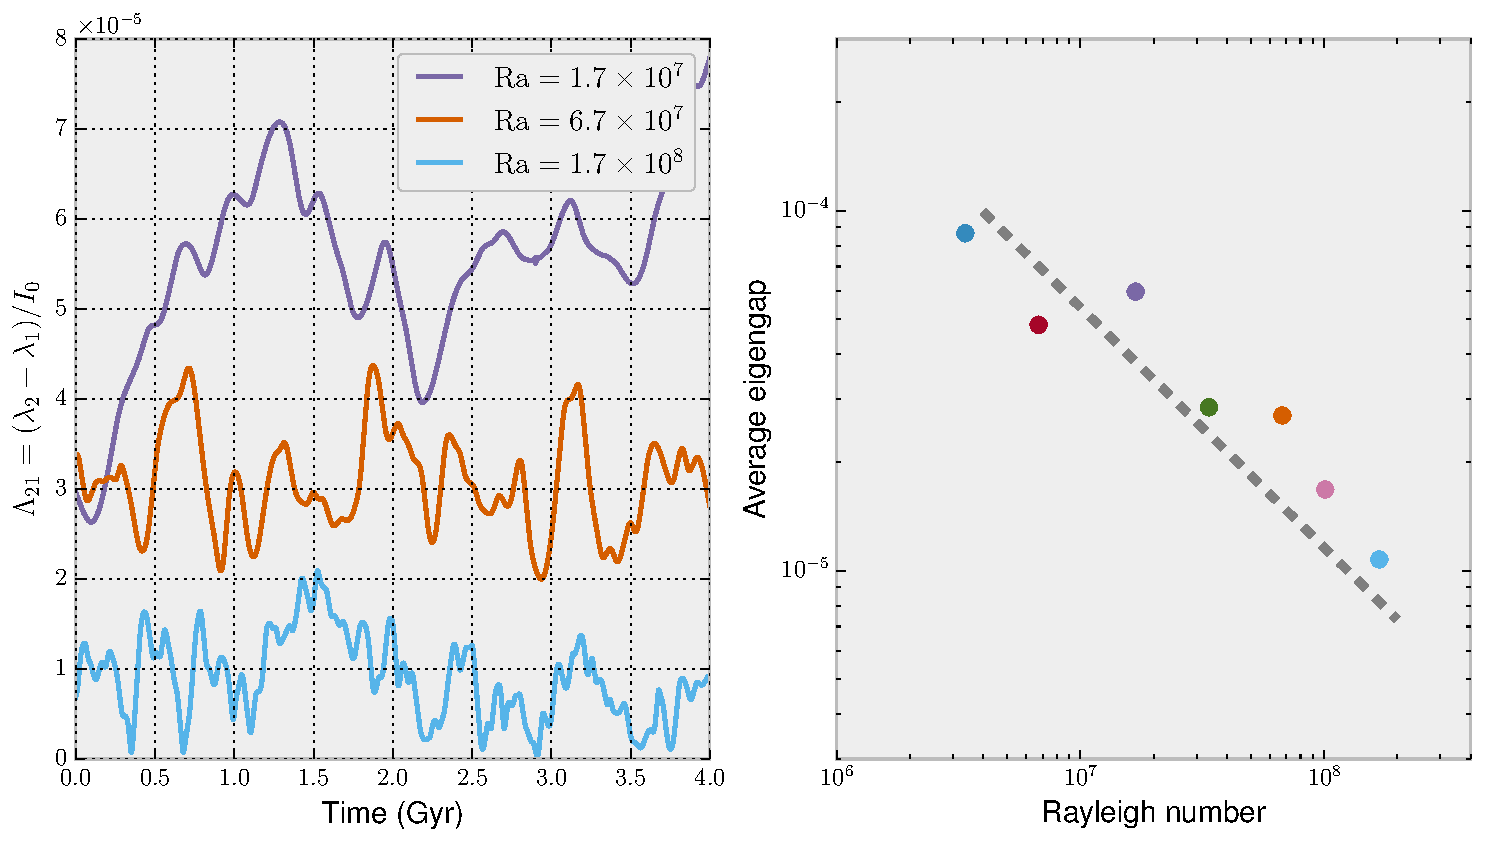
\includegraphics[width=0.9\textwidth]{figures/eigengap.pdf}
\caption[Normalized difference between convective moments of inertia in the mantle.]{ Left: Time series of the normalized difference between moments $\Lambda_{21} = (\lambda_2 - \lambda_1)/I_0$ for convection in a 2D annulus at several different Rayleigh numbers.  As the Rayleigh number increases, the average value of the relative moment decreases due to less low-degree coherence in the temperature structure.  Right:  average value of $\Lambda_{21}$ for the different Rayleigh numbers.  Also shown is a line with slope $\mathrm{Ra}^{-2/3}$, which is predicted from the scaling analysis (the exponent is $-2/3$ instead of $-1$ due to the reduced dimensionality of the simulations).}
\label{fig:eigengap}
\end{figure*}


Fluctuations in the nonhydrostatic moment of inertia are caused by density variations 
due to the temperature fluctuations in the mantle and their spatial structure:

\begin{equation}
C_{ij} = \int_{V_H} \rho_0 \alpha (T-T_0) \left( r_q r_q \delta_{ij} - r_i r_j \right) \,dV
\label{eq:temperature_fluctuations}
\end{equation}
As discussed in Section~\ref{sec:convective_moment}, these internal density loads may be convolved with their surface responses to get the convective moment of inertia $E_{ij}$.
The surface response is a function of the viscosity structure of the planet and the wavelength and depth of the internal load.
The factor $(1+k^L_f)$ is generally an order-one parameter 
(strictly speaking, dynamic compensation usually makes it less than one, \citep[e.g.][]{richards1984geoid}). 
For the purposes of scaling, it is reasonable to neglect this multiplicative factor.

For thermal convection, the convective part of the moment of inertia $E_{ij}$ is directly related to the degree-two part of the temperature field (see Appendix~\ref{appendix:moments}).
Therefore, an estimate for one specifies the other.
We can expand the temperature structure of the convecting planet with a set of orthonormal basis functions $R_n Y_{lm}$, 
where $Y_{lm}$ are spherical harmonics, $R_n$ are some set of orthogonal radial polynomials, and
$T_{nlm}$ are the coefficients for the expansion which have been normalized by $\Delta T$:
\begin{equation} 
T( r , \theta, \phi, t )  = \Delta T {\displaystyle \sum_{n=0}^\infty \sum_{l=0}^\infty \sum_{m=-l}^{l} } T_{lmn}(t) R_n(r) Y_{lm} (\theta , \phi).
\label{eq:T_series}
\end{equation}
Inserting the temperature expansion~\eqref{eq:T_series} into Equation~\eqref{eq:temperature_fluctuations} results in 
a prefactor of the nondimensional number $\Gamma = \alpha \Delta T$.
Orthogonality of the basis functions for the expansion means that the integral for $C_{ij}$ picks out degree-two 
spherical harmonics in the lateral dimensions, and only the lowest few radial functions $R_n(r)$.
Therefore, of the entire temperature spectrum, only a few of the modes matter for TPW.
We want to estimate the power in those few modes, which we denote by $T_{\text{degree-two}}$ (see Appendix~\ref{appendix:moments} for more detail): 
\begin{equation}
\Lambda_{31} \sim \Gamma T_{\text{degree-two}}.
\end{equation}
The temperature field has been normalized by $\Delta T$ and thus goes between zero and one, therefore the expansion in $T_{lmn}$ is constrained by

\begin{equation}
\max \left( \displaystyle \sum_{n=0}^\infty \sum_{l=0}^\infty \sum_{m=-l}^{l} T_{lmn}(t) R_n(r) Y_{lm} (\theta , \phi) \right) = 1.
\end{equation}
This is a strong constraint, but it gives very little information about the distribution of power across the $T_{lmn}$.  
We can, however, think about the power spectrum in two different regimes: that of steady/quasisteady flow, (relatively low $\mathrm{Ra}$) 
and that of chaotic flow (relatively high $\mathrm{Ra}$).
The structure of thermal convection is primarily controlled by the Rayleigh number.  Once the Rayleigh number is sufficiently high ($\sim10^6$) 
the style of convection changes from steady/quasisteady to chaotic.  Accompanying this transition to chaos is a broadening of the spatial 
and temporal spectra \citep{mclaughlin1982transition}.  

At low Rayleigh number we expect the spectrum of the temperature field to be dominated by only a few low-degree modes which are largely influenced by the aspect ratio.
This spectrum may or may not have a lot of power in the degree-two modes, and does not depend strongly on time.

At high Rayleigh number we expect the shortest lengthscales to be limited by the effects of thermal diffusion,
which tends to wipe out thermal heterogeneity at small scales.  Consequently, there will be little power in modes
with shorter lengthscales than that allowed by diffusion. 
Therefore we expect, to a good approximation, that the infinite sum in Equation~\eqref{eq:T_series} can be truncated at some maximum wavenumber, set by the smallest lengthscale $d$:
\begin{equation}
n_{\text{max}}, l_{\text{max}}, m_{\text{max}} \sim \frac{R}{d}.
\label{eq:max_wavenumber}
\end{equation}
Strictly speaking, convective mixing can produce smaller scales, but the power in these scales
is greatly reduced by diffusion.
Thus total number of modes that are accessible to the system are 

\begin{equation}
N_{\text{modes}} = n_{\text{max}} \times l_{\text{max}} \times m_{\text{max}} \sim \left( \frac{R}{d} \right)^{3}.
\end{equation}
The value of each $T_{lmn}(t)$ will in general be some complex function of time, but for a given style of convection we expect there to be some average value.
For chaotic flow the power should be spread out amongst the modes accessible to it.
We may make the hypothesis that each of the modes are roughly as likely as any of the others, which implies

\begin{equation}
T_{\text{degree-two}}(t) \sim \frac{1}{N_{\text{modes}}} \sim \left( \frac{d}{R}\right)^3.
\end{equation}

Any of a number of scaling laws can provide an estimate for the characteristic length scale of a convecting system which may depending on rheology, geometry, or density structure.
The simplest, based on boundary layer theory \citep{turcotte1967finite}, finds $d/R \sim \mathrm{Ra}^{-1/3}$.
This scaling is roughly a measure of the diffusive lengthscale for the timescale of a convective overturn, consistent
with the cutoff in Equation~\eqref{eq:max_wavenumber}.
It thus furnishes us with an estimate of the power in 
the degree-two part of the field as a function of Rayleigh number:

\begin{equation}
T_{\text{degree-two}}(t) \sim \mathrm{Ra}^{-1}.
\label{eq:degree_two_of_ra}
\end{equation}

We performed a series of numerical simulations of mantle convection at different Rayleigh numbers to test this scaling.
We used the mantle convection software \texttt{ASPECT} \citep{kronbichler2012high}, based on the finite element library \texttt{deal.II} \citep{dealII82},
which allows for flexible implementation of different rheologies, geometries, and postprocessors.
In order to test a wide range of Rayleigh numbers, we ran the simulations in a 2D annulus, tracking the eigenvalues of the 
moment of inertia tensor and integrating Equation~\eqref{eq:liouville_ode} in time.
For the 2D simulations there is a reduced dimensionality when calculating the number of modes,
so $N_\text{modes} \sim \left(R/d \right)^2$.  This leads us to a scaling of $T_{\text{degree-two}} \sim \mathrm{Ra}^{-2/3}$, 
which is shown as a dashed line in Figure~\ref{fig:eigengap}.
This result has a simple interpretation.
As the Rayleigh number of the system increases, the smallest lengthscale of convective features gets smaller.
The total power in the temperature field is spread across a larger spectrum, leaving less total power for the degree-two part, which is what drives TPW.


With an estimate for the power in the degree-two part of the temperature field, we may finally estimate $\Lambda_{ij}$:
\begin{equation}
\Lambda_{ij} \sim \frac{\Gamma}{\mathrm{Ra} }.
\label{eq:lambda_estimate}
\end{equation}
Other power spectra for the temperature field are possible. Isoviscous models tend to be ``bluer,'' (dominated by small wavelengths) 
and models with viscosity stratification tend to be ``redder'' (dominated by long wavelengths) \citep{richards1999polar}.
Present day Earth seems to have a fairly ``red'' spectrum, with large low-degree seismic anomalies due to 
Cenozoic subduction history and the lower mantle LLSVPs \citep{dziewonski2010mantle}.
Nevertheless, at high Rayleigh number the expectation is that the power will be distributed across many length scales.


\subsection{An estimate for the angular mismatch angle ($\theta$)}
\label{sec:theta}

Convection can drive both growth and decay in the mismatch angle ($\theta$) between the current rotation axis and the principal axis of the convective moment. 
This parameter is crucial for the rate of TPW, as previously noted in Equation~\eqref{eq:scaled_rotation}.  
Much of the debate around the existence and magnitude of TPW on Earth comes down to the question of how big $\theta$ can be \citep{kirschvink1997evidence, steinberger1997changes}.

Two processes control the evolution of $\theta$. Its growth occurs through perturbations in the convective moment and 
its decay occurs by relaxation of the pole towards the maximum moment of inertia.
We can explore these two effects by converting Equation~\eqref{eq:liouville_ode}
from the body-fixed frame to the $\mathbf{E}$-frame (recall that $\mitbf{\Omega}$ defines
the rotation of the body-fixed frame relative to inertial space in Equation~\eqref{eq:euler}).
The $\mathbf{E}$-frame rotates slowly with respect to the geographic frame, 
which we describe by the rotation vector $\mathbf{\Psi}$. 
(To be explicit in our discussion we let $\mitbf{\Psi}$ define the rotation of the $\mathbf{E}$-frame in the geographic frame, 
although this choice is arbitrary as long as we are consistent). The time derivatives of $\mitbf{\omega}$ in the two frames are related by 
\begin{equation}
\dot{\mitbf{\omega}} = \dot{\mitbf{\omega}}^\prime + \mathbf{\Psi}\times \mitbf{\omega}^\prime.
\end{equation}
where primes are used to define quantities in the $\mathbf{E}$-frame. Rearranging gives 
\begin{equation}
\dot{\mitbf{\omega}}^{\prime} = \dot{\mitbf{\omega}} - \mathbf{\Psi}\times \mitbf{\omega}^\prime.
\end{equation}
We now substitute for $\dot{\mitbf{\omega}}$ from Equation~\eqref{eq:liouville_ode}, 
making the additional assumption that the geographic and $\mathbf{E}$-frames are momentarily aligned. 
This assumption is not a serious restriction because our goal is simply to relate the time derivatives of $\mitbf{\omega}$ in the two frames, 
rather than track the evolution of $\mitbf{\omega}$ over time. The expression for $\dot{\mitbf{\omega}}$ becomes
\begin{equation}
 \dot{\mitbf{\omega}}^\prime  = \frac{1}{(C-A)T_1} \left[ \mathbf{E}^\prime \cdot \mitbf{\omega}^\prime - \left( \mitbf{\omega}^\prime \cdot \mathbf{E}^\prime \cdot \mitbf{\omega}^\prime  \right) \mitbf{\omega}^\prime \right] - \mathbf{\Psi}\times \mitbf{\omega}^\prime.
\label{eq:liouville_ode_new_frame}
\end{equation}
The advantage of expressing the rate of TPW in the $\mathbf{E}$-frame is that the entire equation
may be written in terms of the principal moments $\lambda_i$ and the angles from the principal axes.
As in Equation~\eqref{eq:simple_milankovitch}, we make the simplifying assumption that 
$\mitbf{\omega}^{\prime}$ lies in $\mathbf{e}_1^{\prime}-\mathbf{e}_3^{\prime} $ plane (as shown in Figure~\ref{fig:reference_frames}). 
In this case the orientation of $\mitbf{\omega}^\prime$ is defined by colatitude $\theta$ and longitude $\phi=0$. 
The colatitude $\theta$ is precisely the angular misalignment that specifies the rate of TPW in Equation~\eqref{eq:simple_milankovitch}.
We furthermore specify the orientation of $\Psi$
using colatitude $\beta$ and longitude $\gamma$ (see Figure~\ref{fig:reference_frames}).

The time derivative of the unit vector $\mitbf{\omega}^{\prime}$ defines the changing orientation of the rotation axis in the $\mathbf{E}$-frame. 
We can express this changing orientation in terms of changes in angles $\theta$ and $\phi$. The change in colatitude is
\begin{equation}
\dot{\theta} = 
-\frac{1}{2(C-A) T_1}\sin{2\theta} ( \lambda_3 - \lambda_1) - \vert \mitbf{\Psi} \vert \sin\beta \sin\gamma.
\label{eq:theta_competition}
\end{equation}
where $\mitbf{\Psi}$ is expressed in terms of its amplitude $|\mitbf{\Psi}|$ and its orientation angles $\beta$ and $\gamma$.
Equation~\eqref{eq:theta_competition} captures the essential competition between growth and decay of the mismatch angle.
The first term acts to reduce $\theta$ via TPW, while the second term can increase (or decrease) it via
relative motion between the geographic frame and the principal axes of the $\mathbf{E}$-frame.
Comparison with Equation~\eqref{eq:simple_milankovitch} shows that, when $\vert \mitbf{\Psi} \vert$ is zero,
then the rate of TPW $\vert \dot{\Theta} \vert$ is identical to $\vert \dot{\theta} \vert$.
Conversely, when the rate of TPW is very slow (i.e. $\vert \dot{\Theta} \vert \sim 0$), 
then $\vert \dot{\theta} \vert \sim \vert \mitbf{\Psi} \vert$, so the evolution of $\theta$ is driven mostly by $\mitbf{\Psi}$. 
For the purposes of scaling we will omit the orientation factor $\sin \beta \sin \gamma$ and focus on $|\mitbf{\Psi}|$.
In order for the TPW rate to be large, the growth of $\theta$ via $\vert \mitbf{\Psi} \vert$ must, 
at least occasionally, be larger than its decay.

An estimate for $\vert \mitbf{\Psi} \vert$ must concern the stability of the convective moment of inertia. 
Convection is continuously redistributing mass throughout the mantle, which will perturb the convective moment of inertia.  
If the convective moment is stable to small perturbations, then $\vert \mitbf{\Psi} \vert$ should be small, so
 $\theta$ will never have the opportunity to grow.
However, if $\mathbf{E}$ is not stable to perturbations, then $|\mitbf{\Psi}|$ can be large and $\theta$ can grow up to $90^\circ$. 
Given a random perturbation to $\mathbf{E}$, we would like to give a bound on the size of changes in the orientation of the principle axes. 
This may be done by application of a theorem due to \citet{davis1970rotation}.

Let $\delta$ be the size of the perturbation to the convective moment of inertia tensor after some time interval $\Delta t$, and let $\lambda_3 \ge \lambda_2 \ge \lambda_1$ be the eigenvalues of that tensor.  The corresponding rotation of the principal axes is defined by the angle $\xi$. A bound on $\xi$ is given by 
\begin{equation}
\vert \sin(2 \xi) \vert \le \frac{ 2 \vert \delta \vert}{ \displaystyle \min_{i \neq j} \vert \lambda_i - \lambda_j \vert }.
\label{eq:kahan}
\end{equation} 
That is to say, if there is a large difference between the eigenvalues, this stabilizes axes to perturbations.  
If, however, there is a small difference between the eigenvalues (i.e., they are nearly degenerate), then perturbations can cause large rotations of the principal axes.
This is illustrated schematically in Figure~\ref{fig:perturb}.
\citet{evans1998true} described a situation where the convective moment of inertia of Earth is prolate, with the
maximum and intermediate moments of inertia nearly equal.
He argued that perturbations in this case would result in TPW paths that are approximately
on the great circle path between the intermediate and maximum axes.
This behavior is a consequence of the instability described in Equation~\eqref{eq:kahan}.

We may arrive at a simple estimate for $|\mitbf{\Psi}|$  
by differentiating Equation~\eqref{eq:kahan}, tentatively holding $\vert \lambda_i - \lambda_j \vert$ fixed:
\begin{equation}
\vert \mitbf{\Psi} \vert \sim \vert \dot{\xi} \vert \le \frac{ \vert \dot{\delta} \vert}{ \displaystyle \min_{i \neq j} \vert \lambda_i - \lambda_j \vert }.
\label{eq:grow_perturbation}
\end{equation} 
As noted previously, $|\mitbf{\Psi}|\sim |\dot\theta |$ when the rate of TPW is small and the angular misalignment $\theta$ is small. 
Consequently, we can interpret Equation~\eqref{eq:grow_perturbation} as a bound on how fast $\theta$ can grow.

\begin{figure*}
\centering
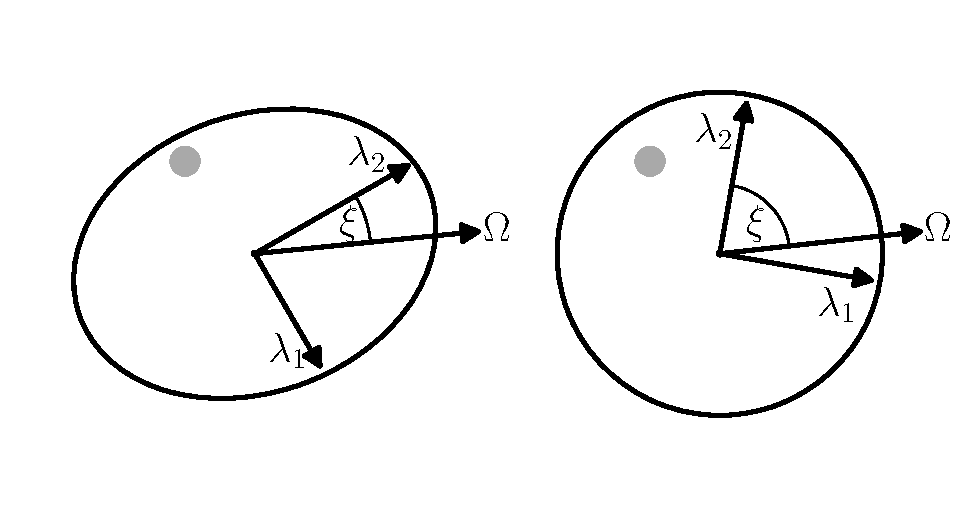
\includegraphics[width=0.9\textwidth]{figures/perturb.pdf}
\caption[Graphical demonstration of the $\sin{2 \xi}$ theorem of \citet{davis1970rotation}.] {Graphical demonstration of the $\sin{2 \xi}$ theorem of \citet{davis1970rotation}.  Two spheroidal bodies with eigenvalues $\lambda_2 > \lambda_1$ start out with the rotation axis $\Omega$ aligned with the $\lambda_2$ axis. However, on the left the eigengap $\lVert \lambda_2 - \lambda_1 \rVert$ is large, while on the right it is small.  A negative mass perturbation is instantaneously added to both bodies, which effects a small rotation of the principal axes on the left, but a large one on the right.}
\label{fig:perturb}
\end{figure*}

The quantity $(\lambda_i-\lambda_j)$ which appears in the denominator of these equations is precisely the same as the quantity which we estimated in the previous section to scale with $\sim \mathrm{Ra}^{-1}$.
Therefore, as the Rayleigh number increases, the characteristic gap between the eigenvalues of the convective moment becomes smaller.  
Additionally, the timescale of fluctuations in these values goes down. 
Overall, this makes the principal axes of high Rayleigh number systems much less stable.
This is consistent with the result of \citet{richards1999polar}.

In the limit that the eigengap becomes zero, the rotation of the principle axes can be arbitrary. 
This essentially corresponds to the hypothesized ``inertial interchange true polar wander'' \citep{kirschvink1997evidence}, where 
the mismatch angle is $90^\circ$. However, the eigengap does not need to be zero for there to be large displacements polar wander, 
and if it does go to zero, the wander does not need to be $90^\circ$.

Figure~\ref{fig:misfit} shows a representative timeseries for annular convection, where 
we track the eigenvalues of the moment of inertia and integrate Equation~\eqref{eq:liouville_ode} in time.
Since it is a 2D model, the spin axis may be represented by a single angle.
When the eigengap gets small, the misfit angle becomes much larger, and the rate of polar wander becomes much faster.
At $\sim$1 Gyr into the model run the eigengap goes to zero, and the misfit angle goes to approximately $90^\circ$, 
an IITPW event. But there are several other events where the eigengap becomes small, and there are 
still large TPW events associated with them.
For example, at $\sim$0.3 Gyr the eigengap dips, with an associated large TPW event, even though
there is technically no interchange of the axes.

We suggest, then, that $90^\circ$ IITPW events are simply a special case of a broad class of events which can occur
when the principal moments are close to each other. 
Furthermore, a more vigorously convecting planet is much more likely to experience rapid TPW events
as it has a lower characteristic gap between principal moments and the gap is much more likely to go to zero.

\citet{tsai2007theoretical} suggested that interchanges in the principal moments are unlikely to produce large
TPW events, since (1) during an inertial interchange the total moment of inertia anomaly is small, and
(2) the TPW event can only asymptotically approach 90$^\circ$.
This is true for the case of a single interchange. However, we argue that this is overly restrictive
for our generalization of IITPW.
Our numerical experiments show that in a vigorously convecting system the principal moments can
interchange, or almost interchange, quite rapidly, and the perturbation sizes can be large soon after an interchange.
Furthermore, the location of the principal axes need not stay put during a TPW event,
which can lead to extended polar wandering of distances greater than 90$^\circ$.

\begin{figure*}
\centering
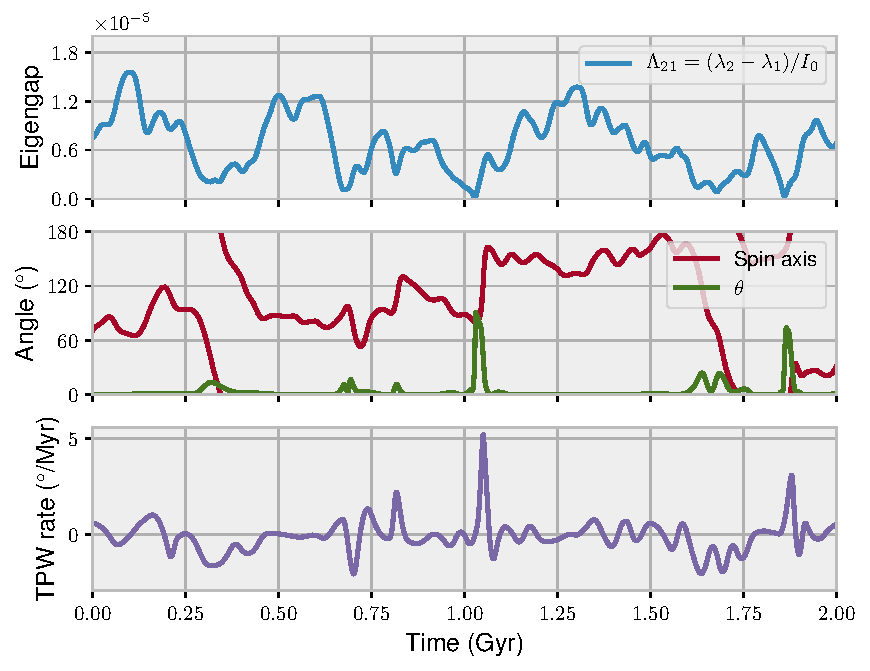
\includegraphics[width=0.9\textwidth]{figures/misfit.pdf}
\caption[Principal moments and mismatch angle in a convecting matle.]{Top: Time series of principal moments for 2D annular convection at $\mathrm{Ra}\sim10^8$.  Bottom: Time series of spin axis and mismatch angle $\theta$.  When the two moments are close to each other (small eigengap), the mismatch angle becomes large, and the rate of polar wander is significantly larger. At $\sim$1 Gyr the gap goes to zero and there is a nearly $90^\circ$ TPW event, with $\sim80^\circ$ degrees of polar wander in $\sim$30 Myr. However, there are several other large TPW events which happen when the eigengap is small.}
\label{fig:misfit}
\end{figure*}


\section{Discussion}
\label{sec:discussion}

The preceding results clarify the complex relationship between the Rayleigh number, $m$, and the rates of TPW for a convecting planet.
As mantle convection redistributes mass in the planet's interior, the spin axis moves around to stay aligned with the principal axes of the convective moment of inertia. 
There is a constant competition between growth of the mismatch angle $\theta$ through 
Equation~\eqref{eq:grow_perturbation} and its relaxation through TPW.
\citet{goldreich1969some} envisioned an analogy of beetles crawling on the surface of the globe, with
the spin axis trying to keep up with the instantaneous figure axis set by the beetles.
Our analysis begins to answer the questions ``how big are the beetles?'' and ``how fast are they crawling?''

We may plug in the estimate for $\Lambda_{ij}$ (Equation~\eqref{eq:lambda_estimate}) into Equation~\eqref{eq:simple_milankovitch} to find the strikingly simple expression
\begin{equation}
\frac{\kappa}{R^2} \; \dot{\Theta} \sim -\frac{1}{m} \sin{2 \theta}.
\label{eq:simplest_milankovitch}
\end{equation}
Surprisingly, $\Gamma$ and $\mathrm{Ra}$ have completely dropped from the prefactor in the scaling. 
Response timescales for relaxation of the mismatch angle go down at high Rayleigh numbers.
At the same time, however, coherence in the temperature structure goes down, reducing the amount of power in the degree-two part of the field responsible for driving TPW.
That these two effects cancel is something of a coincidence due to the simple estimate of the smallest lengthscales of the problem.
Scalings for lengthscales of convection in fluids with temperature dependent viscosity \citep[e.g.][]{solomatov1995scaling} or pseudoplastic rheology \citep[e.g.][]{korenaga2010scaling} have different functional dependencies on $\mathrm{Ra}$ or additional nondimensional parameters.
However, a common feature in most scalings is that typical lengthscales are still some power-law of Rayleigh number $d \propto \mathrm{Ra}^{-\beta}$.
With this form, our scaling for TPW rate has the following dependence on $\mathrm{Ra}$:
\begin{equation}
\frac{\kappa}{R^2} \; \dot{\Theta} \sim -\frac{\mathrm{Ra}^{1-3\beta}}{m} \sin{2 \theta}.
\label{eq:simplest_milankovitch_defer_scaling}
\end{equation}
In general, $\beta$ is some small number between one-fourth and one-third, so we expect that more complicated estimates for 
$d(\mathrm{Ra})$ will still result in a weak dependence of the prefactor in Equation~\eqref{eq:simplest_milankovitch_defer_scaling} 
on the Rayleigh number.

We then suggest that the most important parameters are $m$, which acts as the brakes on the system, and the mismatch angle $\theta$.
Whereas the prefactor $\mathrm{Ra}^{1-3\beta}$ in Equation~\eqref{eq:simplest_milankovitch_defer_scaling} has a weak dependence on $\mathrm{Ra}$, 
the misalignment angle $\theta$ is expected to be strongly dependent on it.

Indeed, we can identify two endmember behaviors of Equation~\eqref{eq:simplest_milankovitch_defer_scaling}.
When convection is not sufficiently chaotic to create a large $\theta$ we are in the regime where the planet's rotation axis closely tracks that of the convective moment.
This is the regime considered in \citet{steinberger1997changes}, \citet{roberts2007cause}, and \citet{zhong2007supercontinent}, and can be considered the ``slow TPW'' regime.
When convection is more chaotic, however, there may be large excursions in $\theta$, 
which are driven by large values for $|\mitbf{\Psi}|$ when $(\lambda_i - \lambda_j)$ is small, according to Equation~\eqref{eq:grow_perturbation}. 
In this case a dramatic increase in the rate of TPW is possible.
If $\theta=90^\circ$, this corresponds to IITPW \citep{kirschvink1997evidence}.  
This, however, is a special case in the large $\theta$, ``fast TPW'' regime.

As an example, we may consider the early Earth, when the mantle was presumably hotter and less viscous, leading to a 
higher Rayleigh number. We would then predict that convection was more vigorous, leading to 
a less stable $\theta(t)$, and thus more TPW and more frequent ``fast TPW'' events.

For Cenozoic Earth we can substitute direct estimates of the important parameters into Equation~\eqref{eq:simple_milankovitch}.
Typical values for the time constant $T_1$ are of order $30 \, \mathrm{kyr}$ \citep{ricard1993polar}.
Estimates of the present day non-hydrostatic moment of inertia (due to mantle density anomalies, corresponding to $\Lambda_{31}I_0$ in the preceding scaling)
are in the neighborhood of $10^{-5} I_0$, while the hydrostatic moment of inertia (corresponding to $C-A$) is $3 \times 10^{-3} I_0$ \citep{chambat2001mean}.
A key question is whether convection is sufficiently chaotic to enter the large $\theta$ regime. 
\citet{richards1997explanation} have argued that the convective planform of Earth has been stable for the last
few hundred million years. On the other hand, we know that there have been large reorganizations of that planform 
during Earth history, so this recent geologic stability may not hold in general \citep{evans2003true}.
Our numerical simulations show that large values for $\theta$ are possible in a vigorously convecting mantle.
Allowing for such a large mismatch angle ($\theta = 45^\circ$) we may estimate the maximum polar wander rate
\begin{equation}
\max ( \dot{\Theta} ) = \frac{(\lambda_3-\lambda_1)}{(C-A)}\frac{1}{T_1} \sim 6^\circ / \mathrm{Myr},
\end{equation}
which corresponds to about 66 cm/yr 90$^\circ$ from the TPW axis.
This is similar to the rates discussed by \citet{cambiotti2011new}, (though our rate is larger since we allow for the
possibility of a larger mismatch angle), and is within the range suggested by some interpretations of paleomagnetic data.
The bulk viscosity of Earth's mantle is uncertain by up to a factor of ten \citep{mitrovica2004new},
which results in a corresponding uncertainty for the relaxation time $T_1$ and the maximum polar wander rate.

Thus far we have restricted our discussion to planets with lithospheres lacking long-term elastic strength.
For this case the long-time limit of the planetary figure is coaxial with the convective 
moment of inertia. This assumption is not necessarily true in all cases.
Earth's lithosphere is pervasively fractured and hydrated, and may not have much strength when subjected to rotational changes on geologic timescales.
However, a planet with a stagnant lid (such as Mars) may have considerable strength, preventing the figure of the planet 
from reaching the fluid limit of Equation~\eqref{eq:fluid_love}.

The theory of TPW response for the case of elastic lithospheres has been developed in, among other places, 
\citet{matsuyama2006rotational}, \citet{creveling2012mechanisms}, and \citet{chan2014time}.
The formalism developed in Section~\ref{sec:scaling} can still be applied to this case, 
though the response to internal variations in the moment of inertia becomes more limited 
(and potentially richer, as in the oscillatory motions suggested by \citet{creveling2012mechanisms}).

\section{Conclusion}
We have developed a framework for discussing the rates of true polar wander for a convecting planet 
from a perspective of scaling and fluid dynamics.
We identified a small number of dimensionless parameters which describe the system, and showed how they affect the overall dynamics of the system.

The most important parameters are the Rayleigh number and $m$, which acts as a damper to TPW.
The dependence on the Rayleigh number is more complicated, since it is a control on both the forcing 
of TPW and the response, which act in opposite directions.
Overall, however, we expect that more vigorously convecting planets should be less rotationally stable, and experience more TPW.
This perspective allows us to consider not only the polar wandering of Phanerozoic Earth,
but also allows us to hypothesize about polar wandering during the Archean and Proterozoic, or 
on other planetary bodies.

%\section*{Acknowledgments}
%This work was supported by National Science Foundation grant EAR-1246670. We thank Yanick Ricard for careful and constructive comments that greatly improved the paper.
%We thank the Computational Infrastructure for Geodynamics (geodynamics.org) which is funded by the National Science Foundation under award NSF-0949446.

%\section*{Bibliography}
%\bibliographystyle{elsarticle-harv} 
%\bibliography{tpw_rate}


%\appendix

\section{Degree-two moments}
\label{appendix:moments}

There is a connection between the moment of inertia of a rotating object and the degree-two density structure.
The moment of inertia tensor may be written in index notation
\begin{equation}
I_{ij} = \int_V \rho \left( r_q r_q \delta_{ij} - r_i r_j \right) dV
\label{eq:inertia}
\end{equation}
where $\mathbf{r}$ is the Eulerian coordinate, $\rho$ is the density, and $V$ is the volume of the material.  
It is useful to enter the principal axes of the moment of inertia:
\begin{equation}
\mathbf{I} = \mathbf{1} \begin{bmatrix}
\lambda_1 \\ \lambda_2 \\ \lambda_3
\end{bmatrix} = 
\mathbf{1} \begin{bmatrix}
\int_V \rho (y^2+z^z) dV\\
\int_V \rho (x^2+z^2) dV\\
\int_V \rho (x^2+y^2) dV
\end{bmatrix}
\end{equation}
where $\mathbf{1}$ is the identity matrix, and $\lambda_1$, $\lambda_2$, and $\lambda_3$ are the principal moments.
From Equation~\eqref{eq:polar_wander_rate} we see that the important quantities are the differences between the 
principal moments, $(\lambda_3-\lambda_1)$, $(\lambda_3-\lambda_2)$ and $(\lambda_2-\lambda_1)$.
These quantities may be rewritten in terms of degree-two real spherical harmonics \citep[e.g.][]{dahlen1999theoretical}.
The relevant (fully normalized) harmonics are, in Cartesian coordinates:
\begin{equation}
\begin{aligned}
Y_{20} &= \frac{1}{4} \sqrt{\frac{ 5}{\pi}} \frac{ 2 z^2 - x^2 - y^2}{r^2} \\ 
Y_{22} &= \frac{1}{4} \sqrt{\frac{15}{\pi}} \frac{ x^2 - y^2}{r^2}.
\end{aligned}
\end{equation}
Solving for $( \lambda_i - \lambda_j )$ in terms of these harmonics, we find
\ifdetail

It is useful to define unnormalized versions of the spherical harmonics as intermediate products:
\begin{equation}
\begin{aligned}
Y_{20}^* &= 2 z^2 - x^2 - y^2 &= 4 \sqrt{ \frac{\pi}{5} } r^2 Y_{20} \\ 
Y_{22}^* &= x^2 - y^2 &= 4 \sqrt{ \frac{\pi}{15} } r^2 Y_{22}.
\end{aligned}
\end{equation}
These make it easy to rewrite the differences between the $\lambda_n$:
\begin{equation}
\begin{aligned}
(\lambda_2 - \lambda_1) &= \int_V \rho Y_{22}^* \, dV \\
(\lambda_3 - \lambda_1) &= \frac{1}{2} \int_V  \rho \left( Y_{22}^* - Y_{20}^* \right) dV \\
(\lambda_3 - \lambda_2) &= -\frac{1}{2} \int_V \rho \left( Y_{22}^* + Y_{20}^*  \right) dV. \\
\end{aligned}
\end{equation}
Substituting back in for the normalized spherical harmonics we find
\fi
\begin{equation}
\begin{aligned}
(\lambda_2 - \lambda_1) &= 4 \sqrt{\frac{\pi}{15} } \int_V   \rho r^2  Y_{22} \,dV \\
(\lambda_3 - \lambda_1) &= 2 \sqrt{ \frac{\pi}{15} } \int_V  \rho r^2 \left( Y_{22} - \sqrt{3} Y_{20} \right) dV \\
(\lambda_3 - \lambda_2) &= -2 \sqrt{ \frac{\pi}{15} } \int_V  \rho r^2 \left( Y_{22} + \sqrt{3} Y_{20} \right) dV. \\
\label{eq:degree_two_moments}
\end{aligned}
\end{equation}
Up to the normalization constants, these expressions are identical to multipole expansions, 
picking out the degree-two part of the density field laterally, and low-order polynomials radially.
When density is a function of temperature, we can insert the equation of state, Equation~\eqref{eq:eos}, into 
Equation~\eqref{eq:degree_two_moments} and integrate over a reference spherical volume $V_S$.
This allows us to drop the terms which integrate to zero due to the orthogonality of spherical harmonics, and we are left with:
\begin{equation}
\begin{aligned}
(\lambda_2 - \lambda_1) &= -4 \sqrt{\frac{\pi}{15} } \alpha \rho_0 \int_{V_S} T r^2  Y_{22} \,dV \\
(\lambda_3 - \lambda_1) &= -2 \sqrt{ \frac{\pi}{15} } \alpha \rho_0 \int_{V_S} T r^2 \left( Y_{22} - \sqrt{3} Y_{20} \right) dV \\
(\lambda_3 - \lambda_2) &= 2 \sqrt{ \frac{\pi}{15} } \alpha \rho_0 \int_{V_S}  T r^2 \left( Y_{22} + \sqrt{3} Y_{20} \right) dV. \\
\label{eq:degree_two_moments_of_temperature}
\end{aligned}
\end{equation}
We normalize the differences in eigenvalues by the reference moment $I_0$:
\ifdetail
\begin{equation}
\begin{aligned}
\int_{V_S} \rho_0 \frac{2 r^2 - Y_{20}^*}{3} &= \int_{V_S} \rho_0 (x^2 + y^2) dV = I_0 \\
\end{aligned}
\end{equation}
\begin{equation}
I_0 = \frac{2}{3} \int_{V_S} \rho_0 r^2 \left(1 - 2 \sqrt{\frac{\pi}{5}} Y_{20}\right) \,dV
\end{equation}
\fi
\begin{equation}
I_0 = \frac{2}{3} \int_{V_S} \rho_0 r^2 \,dV.
\end{equation}
\ifdetail
\begin{equation}
\begin{aligned}
\Lambda_{21} &= \alpha \Delta T \frac{-6 \sqrt{\frac{\pi}{15} } \int_{V_S} T^\prime r^2  Y_{22} \,dV}{\int_{V_S} r^2 \, dV} \\
\Lambda_{31} &= \alpha \Delta T \frac{-3 \sqrt{ \frac{\pi}{15} } \int_{V_S} T^\prime r^2 \left( Y_{22} - \sqrt{3} Y_{20} \right) dV}{\int_{V_S} r^2 \, dV}\\
\Lambda_{32} &= \alpha \Delta T \frac{3 \sqrt{ \frac{\pi}{15} }  \int_{V_S}  T^\prime r^2 \left( Y_{22} + \sqrt{3} Y_{20} \right) dV}{\int_{V_S} r^2 \, dV} \\
\end{aligned}
\end{equation}
\begin{equation}
\begin{aligned}
\Lambda_{21} &= \Gamma \frac{-6 \sqrt{\frac{\pi}{15} } \int_{V_S^\prime} T^\prime {r^\prime}^2  Y_{22} \,dV^\prime}{\int_{V_S^\prime} {r^\prime}^2 \,dV^\prime} \\
\Lambda_{31} &= \Gamma \frac{-3 \sqrt{ \frac{\pi}{15} } \int_{V_S^\prime} T^\prime {r^\prime}^2 \left( Y_{22} - \sqrt{3} Y_{20} \right) dV^\prime}{\int_{V_S} {r^\prime}^2 \, dV^\prime}\\
\Lambda_{32} &= \Gamma \frac{3 \sqrt{ \frac{\pi}{15} }  \int_{V_S^\prime}  T^\prime {r^\prime}^2 \left( Y_{22} + \sqrt{3} Y_{20} \right) dV^\prime}{\int_{V_S} {r^\prime}^2 \, dV^\prime} \\
\end{aligned}
\end{equation}
\fi
Dividing Equation~\eqref{eq:degree_two_moments_of_temperature} by $I_0$ and nondimensionalizing 
the integrals results in a factor of $\Gamma = \alpha \Delta T$ and a normalized set of 
degree-two coefficients for the temperature field, which we abbreviate as $T_{\text{degree-two}}$:
\begin{equation}
\Lambda_{ij} \sim \Gamma T_{\text{degree-two}}.
\end{equation}

%%ENDCLIP

\end{document}
\endinput
